%%%%%%%%%%%%%%%%%%%%%%%%%%%%%%%%%%%%%%%%%%%%%%%%%%%%%%%%%%%%%%%%%%%%%%%%%%%%%%%%%%%%%
% Aggiunta di un termine:
% --------------------------
% 	- Aggiungi una subsection del termine:
% 		\subsection{Termine} \index{Termine} % alt{forma alternativa,altra,altra}
%		Descrizione del termine.
%	- La parte % alt{...,...} serve allo script nel caso ci siano forme alternative
%	  della stessa parola, ad esempio plurali.
% 	- Se ha una fonte, mettila nella sezione finale (es. url, doc, ecc)
%
%	- \hyperref[label]{termine}
%
%%%%%%%%%%%%%%%%%%%%%%%%%%%%%%%%%%%%%%%%%%%%%%%%%%%%%%%%%%%%%%%%%%%%%%%%%%%%%%%%%%%%%
% Alla consegna
% --------------------------
%	- Va ricreato il file esterno dell'indice.
%    	Comando in TexStudio: Strumenti --> Indice
%	- Verificare che l'indice sia aggiornato correttamente.
%	- Nella repo ci vanno solo i file .tex e .idx
%
%%%%%%%%%%%%%%%%%%%%%%%%%%%%%%%%%%%%%%%%%%%%%%%%%%%%%%%%%%%%%%%%%%%%%%%%%%%%%%%%%%%%%
%V.I sono i very important, macro argomenti


\documentclass[12pt]{article}

\usepackage{makeidx}
%\usepackage{geometry}
\usepackage[utf8]{inputenc}
\usepackage[italian]{babel}
\usepackage{xkeyval}
\usepackage{graphicx}
\usepackage{url}
\usepackage[colorlinks=true,linkcolor=black,urlcolor=blue]{hyperref}
\usepackage{listings}
\usepackage{xcolor}
\usepackage{float}
\usepackage{subfig} %per due immagini vicine
\usepackage{fancyhdr} %per l'header delle pagine
\usepackage[a4paper,top=2.5cm,bottom=2.5cm,left=2.5cm,right=2.5cm]{geometry}

% \geometry{
% 	a4paper,
% 	total={160mm,225mm},
% 	left=25mm,
% 	top=25mm
% }

\AtBeginDocument{\renewcommand\indexname{Indice analitico}}
\makeindex



\begin{document}

	\begin{titlepage}
		\centering
		\LARGE \textbf{Glossario di Ingegneria del Software} \\
		\small \textbf{a.a. 2018-2019}
	\end{titlepage}

	\newpage
	\begin{center}
		\textbf{Premessa}
	\end{center}
	Questo non è un semplice glossario contenente termine-definizione. È stato creato per essere un ``riassunto'' breve, a punti, contenente tutti gli argomenti principali toccati durante il corso di Ingegneria del Sowftare (parte teorica). Per questo motivo, spesso gli argomenti non sono spiegati in maniera esaustiva e non prevedono proprio tutto quello che c'è da sapere, ma il glossario così inteso è ``un aiuto in più'' (spesso le definizioni sono molto informali). Contiene per lo più appunti presi da me a lezione e integra quasi completamente le slide del corso. In più, sono presenti degli altri concetti ricavati dal libro (Sommerville) e alcuni contenuti provenienti da siti esterni (suggeriti dal prof. come link `` per approfondire'' nella pagina del corso). \par

	Il modo migliore per iniziare a leggere il glossario è guardare per prima cosa i termini segnalati come \emph{enfatizzati}, che sono i macro-argomenti più importanti trattati (come per esempio \emph{ANALISI DEI REQUISITI}) e andare successivamente a tutti i collegamenti contenuti nella sezione (le \underline{parole sottolineate}) che sono altre parole chiave del glossario. In generale, una volta che state leggendo la definizione di un termine, può essere utile vedersi anche i termini a loro annessi. \\
	Se mentre leggete vi perdete e avete bisogno di ritornare velocemente ad una parola, vi consiglio di usare il collegamento ``ritorna all'indice'' presente in alto a sinistra in ogni pagina.

	\setcounter{secnumdepth}{0}
	\setcounter{tocdepth}{1}

	\newpage
	\tableofcontents
	\clearpage
	\printindex \label{index} %stampa l'indice in questa posizione
	\clearpage


	\pagestyle{fancy}
	\fancyhf{}
	\rhead{\hyperref[index]{\color{purple}{Ritorna all'indice}}}
	% \lhead{\textsl{Glossario LC}}
	\lhead{\color{black!75}Glossario L.C.}
	\rfoot{ \thepage}


	\flushright{\hyperref[index]{\color{black!65}{Ritorna all'indice}}}\flushleft

	\section{A} \label{sec:A} 
		
		\subsection{AMMINISTRATORE} \index{Amministratore} \label{amministratore}
		È uno dei \underline{\hyperref[ruoli]{ruoli}} in un progetto. Controlla l'ambiente di lavoro. Si occupa di amministrare le infrastrutture di supporto, risolvere problemi legati alla gestione dei processi, gestire la documentazione di progetto e controllare \underline{\hyperref[versione]{versioni}} e \underline{\hyperref[configurazione]{configurazioni}}.
		
		\subsection{ANALISI DEI REQUISITI} \index{Analisi dei requisiti} \label{analisideirequisiti} %V.I
		L' Analisi dei \underline{\hyperref[requirements]{requisiti}} è lo step dopo lo Studio di fattibilità e tratta sostanzialmente di capire appieno il problema. Riguarda la \underline{\hyperref[qualifica]{qualifica}} e se ne occupa l'\underline{\hyperref[analista]{Analista}} che deve cercare di entrare nell'ottica dell'utente. Lo svolgimento dell'analisi prevede lo studio dei bisogni e delle fonti del dominio applicativo, una prima classificazione dei requisiti, una modellazione concettuale del sistema, l'assegnazione dei requisiti alle varie parti del sistema e la negoziazione con il committente. Dopodiché avviene la redazione del \underline{\hyperref[piano]{Piano}} di qualifica per metodi, tecniche, strumenti, tempi ecc. \\
		
		Le \textit{attività} di analisi sono:
			\begin{itemize}
				\item studiare e definire il problema da risolvere, identificando il prodotto da commissionare (compito del cliente), capendo cosa deve essere realizzato e definendo gli accordi contrattuali;
				\item verificare il costo e la \underline{\hyperref[qualita]{qualità}} in base ai \underline{\hyperref[requirements]{requisiti}} derivanti dal cliente;
				\item (lato fornitore) studio dei bisogni e delle fonti, identificando, specificando e classificando i \underline{\hyperref[requirements]{requisiti}};
				\item (lato fornitore) modellazione concettuale del sistema con partizionamento in componenti (ambiti) a scopo di	allocazione dei requisiti (per esempio con diagrammi d'uso);
				\item (lato fornitore) ripartizione dei requisiti a parti del sistema;
				\item accertare la soddisfacibilità dei requisiti rispetto ai
				vincoli di processo;
				\item assicurare, tramite \underline{\hyperref[tracciamento]{tracciamento}}, che i requisiti concordati siano tutti e soli quelli necessari (tutti i requisiti in AR	soddisfano un particolare bisogno) e sufficienti (tutti i bisogni rilevati nelle fonti sono requisiti in AR);
				\item determinare con il cliente l’utilità strategica dei
				\underline{\hyperref[requirements]{requisiti}} concordati;
				\item adozione di norme redazionali (aiuta a evitare espressioni ambigue) e glossario (aiuta a garantire terminologia consistente);
				\item uso di metodi (semi-)formali (aiuta a ridurre
				gli errori di interpretazione) come diagrammi e formule;
			\end{itemize}
		
		I \textit{processi di supporto} implicati da esse sono:
			\begin{itemize}
				\item documentazione, al fine di raccogliere i risultati dello studio di fattibilità e specificare i requisiti;
				\item gestione e \underline{\hyperref[manutenzione]{manutenzione}} dei prodotti, comprendente il \underline{\hyperref[tracciamento]{tracciamento}} dei requisiti, impostazione e gestione della configurazione e dei cambiamenti;
			\end{itemize}
		
		All'interno del nostro progetto possiamo quindi dire di avere diversi prodotti documentali: per \textit{definire} i bisogni (utente e SW) abbiamo il \underline{\hyperref[capitolati]{capitolato d'appalto}}, per \textit{specificare} abbiamo appunto l'Analisi dei Requisiti (che è un documento contrattuale) e lo \underline{\hyperref[studiofattibilita]{Studio di Fattibilità}} (che è un documento interno del fornitore). Per la \textit{ripartizione} dei requisiti invece la questione è molto delicata perchè da qui inizia la \underline{\hyperref[progettazione]{Progettazione}}. Il confine tra Analisi e Progettazione è molto sottile: per esempio, l'\underline{\hyperref[analista]{Analista}} riesce già a vedere dei sotto-problemi che poi però sono compito di chi progetta. 
		
		\begin{figure}[H]
			\centering
			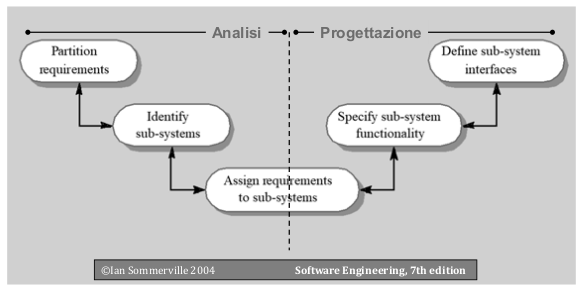
\includegraphics[width=0.8\textwidth]{img/conf}		
			\caption{Confine tra Analisi e Progettazione.}
		\end{figure} 
		
		Ci sono diversi approcci su come procedere per l'Analisi dei Requisiti:
			\begin{itemize}
				\item \textbf{\underline{\hyperref[topdown]{Top-down}}}
				\item \textbf{\underline{\hyperref[bottomup]{Bottom-up}}}
				\item \textbf{Agile} \label{agile}
				Generalmente parto da un'idea di una cosa che già esiste e penso alle funzionalità da poterci aggiungere. É una via di mezzo tra le altre due.
			\end{itemize}	
		
		Le \textit{tecniche} di analisi comprendono:
			\begin{itemize}
				\item l'interazione con il cliente (il cui esito viene documentato), tramite interviste o discussione di scenari;
				\item discussioni creative e collaborative, ovvero \underline{\hyperref[brainstorming]{brainstorming}};
				\item prototipazione,interna (per il fornitore) o esterna (per la discussione con il cliente);
				\item la comprensione del dominio, che prevede: una serie di domande base come \textit{A quali bisogni risponde il prodotto atteso?} e \textit{Quali problematiche d’uso esso comporta}, l'acquisizione delle conoscenze tramite documentazione preesistente e interviste ai potenziali utenti, consolidamento del glossario che raccoglie e definisce i termini chiave del dominio per avere un'interazione ordinata con il committente;
			\end{itemize}
		
		Capita a volte che il progetto venga abbandonato e le principali cause sono:
			\begin{itemize}
				\item \underline{\hyperref[requirements]{requisiti}} incompleti;
				\item insufficiente coinvolgimento del cliente e/o dell’utente (non sono necessariamente la stessa entità);
				\item scarsità di risorse;
				\item attese irrealistiche;
				\item nsufficiente competenza tecnologica e/o metodologica del fornitore;
			\end{itemize}
		
		Mentre gli stati di progresso secondo \underline{\hyperref[semat]{SEMAT}} sono
			\begin{itemize}
				\item \textit{Conceived}: il \underline{\hyperref[committente]{committente}} è identificato e gli \underline{\hyperref[stakeholder]{stakeholder}} vedono sufficienti opportunità per il progetto;
				\item \textit{Bounded}: bisogni macro sono chiari e i meccanismi di \underline{\hyperref[gestionerequisiti]{Gestione dei requisiti}} (\underline{\hyperref[configurazione]{configurazione}} e cambiamento) sono fissati;
				\item \textit{Coherent}: i requisiti sono classificati e quelli essenziali (obbligatori) sono chiari e ben definiti;
				\item \textit{Acceptable}: i requisiti fissati definiscono un sistema soddisfacente per gli stakeholder;
				\item \textit{Addressed}: il prodotto è pronto al rilascio e all'uso;
				\item \textit{Fulfilled}: il prodotto merita la piena approvazione degli stakeholder tanto soddisfa i requisiti;
			\end{itemize}
		
		
		%\subsection{ANALISI DEI RISCHI} \index{Analisi dei rischi} \label{analisirischi} %?
		
		\subsection{ANALISTA} \index{Analista} \label{analista}
		È uno dei \underline{\hyperref[ruoli]{ruoli}} in un progetto. Generalmente sono pochi ma hanno molta influenza sul successo del progetto. Conosce il dominio del problema e ha esperienza professionale, ma raramente segue il progetto fino alla consegna.
		
		\subsection{APPROCCIO} \label{approccio} \index{Approccio}
		Avvicinarsi/predisporsi. Può essere:
			\subsubsection{Sistematico} \label{sistematico}
			ovvero lavorando in maniera metodica (ho un metodo da seguire che mi precede) e rigorosa usando ed evolvendo la \underline{\hyperref[best]{best practice}} [importante il tempo];
			\subsubsection{Disciplinato} \label{disciplinato}
			ovvero seguendo regole fissate;
			\subsubsection{Quantificabile} \label{quantificabile}
			ovvero che permette di misurare \underline{\hyperref[efficienza]{efficienza}} ed \underline{\hyperref[efficacia]{efficacia}};
			
		\subsection{ARCHITECTURE SELECTED}	\index{Architecture Selected}	\label{architectureselected}
		L'architettura viene capita e selezionata, oltre alla selezione delle tecnologie necessarie.	
			
		\subsection{ARCHITETTURA}	\index{Architettura} \label{architettura}
		Si intende architettura logica: è di alto livello (quindi non implementato, concettuale) e consiste nel dividere in parti per massimizzare il parallelismo. Si divide fino a che non se ne trae più vantaggio (fino a che il costo della divisione diventa più un onere che un beneficio).
		Riporta UNA soluzione che soddisfa il cliente.
		L'architettura:
		\begin{itemize}
			\item Decomposta (suggerisce l'idea di top-down) in \underline{\hyperref[componente]{componenti}}.
			\item Ha un'organizzazione: le componenti stanno insieme secondo regole date e ognuna ha un ruolo preciso e collabora.
			\item Definisce le interfacce: qual è il modo in cui le componenti collaborano (parola associata a protocollo (=accordo) perché un'interfaccia si appoggia a un protocollo).
			\item Paradigmi (=come si fa) di composizione: componenti messe insieme secondo regole, limiti, vincoli. Definisce come vengono organizzate.
		\end{itemize}
		Le architetture hanno scelte di paradigmi ed esistono più stili architetturali che determinano l'organizzazione dell'informazione di stato e l'interazione tra le parti
		\underline{\hyperref[qualita]{Qualità}} di una buona architettura: %slide 11/36
		\begin{itemize}
			\item \textbf{Modularità}: (legata a Incapsulazione e Disponibilità) ha l'obiettivo di minimizzare la dipendenza tra parti. Ha due opzioni
			\begin{enumerate}
				\item Suddivide come la pipeline è divisa in stadi;
				\item In modo resiliente, ovvero facendo \textit{information hiding} altrimenti si espone ciò che è "implementation detail" (deve essere ben nascosto perchè altrimenti confonde e dà disagio);
			\end{enumerate}
			\item \textbf{Sufficienza}: deve soddisfare tutti i requisiti, coprire il bisogno;
			\item \textbf{Comprensibilità}: deve essere capita dagli stakeholder, anche perché ci sono diversi stili;
			\item \textbf{Robustezza}: sta in piedi anche se cambio un modulo;
			\item \textbf{Flessibilità}: non deve collassare, deve essere in grado di evolvere (attuando modifiche a costo contenuto);
			\item \textbf{\underline{\hyperref[riuso]{Riusabilità}}}: fare nell'intento che possa essere buono anche per altri in futuro;
			\item \textbf{Efficienza}: senza eccesso di risorse;
			\item \textbf{Affidabilità}: quando c'è bisogno di utilizzarla, fa le cose che deve;
			\item \textbf{Disponibilità}: stare in piedi senza grande bisogno di manutenzione (se una parte è sotto manutenzione, non deve essere interrotto tutto il sistema);
			\item \textbf{Sicurezza rispetto a malfunzionaamenti}: \textit{"safety"}, non ho malfunzionamenti che fanno danno;
			\item \textbf{Sicurezza rispetto a intrusioni}: \textit{"security"}, invulnerabile rispetto alle intrusioni. Mitigare il rischio e massimizzare i vantaggi;
			\item \textbf{Semplicità}: le parti contengono solo il necessario, niente di superfluo;
			\item \textbf{Incapsulazione}: (\textit{Information hiding}) l'interno delle componenti non è visibile dall'esterno, quindi i clienti conoscono solo l'interfaccia, aumenta la manutenibilità e la possibilità di \underline{\hyperref[riuso]{riuso}};
			\item \textbf{\underline{\hyperref[coeso]{Coesione}}}: le parti che stanno insieme hanno gli stessi obiettivi e ognuna ha un ruolo (la coesione si può misurare);
			\item \textbf{Basso accoppiamento}: (l'accoppiamento è la nemesi della coesione, quando viene mossa una parte ne viene conseguentemente mossa anche un'altra) distinte parti che dipendono poco o niente le une dalle altre, ma quando dall'esterno fanno assunzioni su come certe cose stiano all'interno di altre e quando si condividono frammenti delle stesse risorse (bisogna cercare di massimizzare l'indice di utilità e minimizzare l'indice di dipendenza);
		\end{itemize}
		L'architettura definisce i {\underline{\hyperref[ruoli]{ruoli}}}.	
		Tutte le qualità delle caratteristiche attese vanno perseguite. %slide 2/30 verifica e validazione
		Tutto va sottoposto a verifica.
	
		\subsection{AUDIT PROCESS} \index{Audit Process} \label{audit}
		Imporre un andamento e assicurarsi che l'attività che si sta facendo si svolga nel migliore dei modi possibili. Permette di migliorare il \underline{\hyperref[way]{way of working}}. È una revisione \textbf{esterna}.
		
	

	\newpage
	\flushright{\hyperref[index]{\color{black!65}{Ritorna all'indice}}}\flushleft
	\section{B} \label{sec:B}
	
		\subsection{BACKLOG} \index{Backlog} \label{backlog}
		(Chiamato anche "to do") Cose da fare per soddisfare la \textit{user story}, ovvero l'informale descrizione delle caratteristiche che il prodotto software deve avere.
		
		
		\subsection{BASELINE} \index{Baseline}  \label{baseline} 
		Letteralmente "campo base" o "punto d'appoggio" (per evitare situazioni di rischio). È un risultato concreto che risponde alla domanda:"Sì, si può fare". È una risposta buona e possibile in quel dato momento.
		\begin{itemize}
			\item \textbf{Cos'è}: Un progetto software, se si basa su una strategia, avrà una sequenza di obiettivi. Le parti di cui è fatta una baseline (le quali hanno un numero di versioni "as many as needed"), esistono perché assolvono un obiettivo. Una baseline rappresenta quindi un punto di avanzamento consolidato in un dato istante del progetto. Ogni punto di avanzamento viene fissato precedentemente in modo strategico dalla \underline{\hyperref[best]{best practice}}, ma il numero di baseline non è deciso a priori (solo gli obiettivi sono decisi a priori). 
			\item \textbf{A cosa serve}: Dare una base da cui partire per l'avanzamento del progetto.
			\item \textbf{Come si mantiene}: Bisogna decidere come le parti concorrono a formare la baseline tramite versionamento.
			\item \textbf{Come si costruisce}: Tramite configurazione.
		\end{itemize}
		%Ci possono essere più baseline ed essere consecutive. 
		%Insieme di CI (parti che compongono il prodotto che possegono ID, nome, data, autore, registro delle modifiche, stato corrente) consolidato a un dato istante (milestone/data di calendario). 
		
		
		\subsection{BEST PRACTICE} \index{Best practice} \label{best}
		\underline{\hyperref[way]{Modo di fare}} che deve garantire i migliori risultati in specifiche e note circostanze.
		
		
		\subsection{BODY OF KNOWLEDGE} \index{Body of knowledge} \label{body}
		"Corpo"/Insieme di conoscenze che ci ha emancipato.
		
		
		\subsection{BOTTOM-UP} \label{bottomup}
		Concepisco il sistema basandomi dalle ipotetiche parti che possono comporlo. Questo approccio è tipico della \textit{Programmazione ad Oggetti} (esempio di: costruisco il frigo sapendo che esso è un aggregato di reparti). 
		
		
		\subsection{BRAINSTORMING} \index{Brainstorming} \label{brainstorming}
		Pensiero intenso collettivo che fa nascere idee, in cui ognuno parla a turno e non c'è sopraffazione. Durante la discussione, una sola persona scrive. È uno strumento utile per unire debolezze in un'unica forza maggiore.
	
	
		\subsection{BRANCH COVARAGE}	\index{Branch Coverage}	\label{branchcoverage}
		Si occupa di coprire i rami di decisione. Si ha quindi copertura al 100\% quando ciascun ramo del flusso di controllo dell'unità viene attraversato almeno uno volta, ognuno con esito corretto. \\
		Il valore di copertura è determinato dalla complessità di espressioni di decisione (espressioni composte da condizioni contenenti valori booleani).
		%Quando compongo condizioni con operazioni abbiamo Decisione(in rosso). %sono un genio
		
	\newpage
	\section{C} \label{sec:C}
	
		\subsection{CAMMINO CRITICO} \index{Cammino critico} \label{camminocritico}
		Sequenza di attività ordinata con prodotto importante e dipendenze temporali strette. [guardo il cammino di peso massimo].
		
		\subsection{CAPABILITY}	\index{Capability} \label{capability} %(slide 14) Set Lezione del 4/12 - Qualità di processo
		Misura l’adeguatezza di un processo per gli scopi a esso assegnati. È una caratteristica propria del processo e  determina il risultato (in termini di efficienza ed efficacia) raggiungibile per quel processo. Conviene che il livello di capability sia alto, ovvero così seguito da tutti in modo disciplinato, sistematico e quantificabile.
		
		\subsection{CAPITOLATO D'APPALTO} \index{Capitolati d'appalto} \label{capitolati}
		Documento tecnico che descrive in maniera dettagliata tutti i bisogni. In esso vengono spiegate le cose che chi commissiona vuole, nel gergo di una persona normale. Sono interamente responsabilità del cliente e da esso ne conseguono:
			\begin{itemize}
				\item \underline{\hyperref[requirements]{requisiti}} utente, che sono vincoli contrattuali che specificano il \textit{cosa};
				\item \underline{\hyperref[requirements]{requisiti}} software, che specificano il \textit{come};
			\end{itemize} 
		
		\subsection{CICLO DI DEMING} \index{Ciclo di Deming} \label{pdca}
		Il ciclo di Deming (o ciclo di PDCA) è un metodo di gestione iterativo per il controllo e il miglioramento continuo dei processi e dei prodotti suddiviso in 4 fasi:
			\begin{itemize}
				\item \textbf{\underline{\hyperref[pianificazione]{Plan}}} definisce attività, scadenze, ecc. necessari a raggiungere specifici obiettivi di miglioramento;
				\item \textbf{Do} esegue le attività di \textit{Plan};
				\item \textbf{Check} verifica l'esito delle azione di miglioramento rispetto alle attese;
				\item \textbf{Act} consolida il tutto e cerca dei modi per il miglioramento successivo; 
			\end{itemize}
		
		\subsection{CICLO DI VITA} \index{Ciclo di vita} \label{ciclo}
		Si riferisce alla completa durata del prodotto (dal concepimento al ritiro\textit{=fine}) che deve essere garantita. È da vedersi come una macchina a \underline{\hyperref[stato]{stati}} in cui ho una certa sequenza di passaggi da seguire. La transizione tra stati avviene tramite l’esecuzione di
		attività di processi di ciclo di vita. Lo stazionamento in uno stato o transizione viene detta \underline{\hyperref[fase]{fase}}. In seguito al ritiro, il prodotto può essere "rimesso in vita", per questo viene chiamato \textit{ciclo}.
		
		\begin{figure}[H]
			\centering
			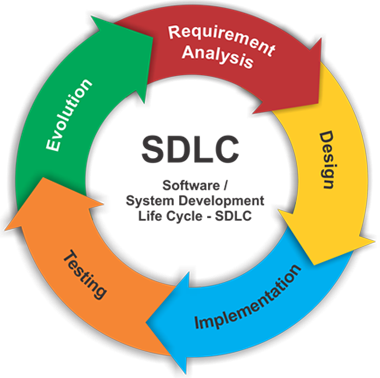
\includegraphics[width=0.5\textwidth]{img/lifecycle}		
			\caption{I 5 stati del ciclo di vita di un prodotto.}
		\end{figure} 
		
		Associare un sistema di \underline{\hyperref[qualita]{qualità}} al modello adottato, aiuta a perseguire conformità nel \underline{\hyperref[progetto]{progetto}} e \underline{\hyperref[maturita]{maturità}} nei processi.	Conoscere il ciclo di vita previsto di un prodotto, aiuta a valutarne preventivamente i tempi, i costi e i rischi. Esistono \underline{\hyperref[processo]{processi}} di ciclo di vita, che specificano le \textit{attività} da svolgere per abilitare le transizioni di stato nel ciclo di vita, e \underline{\hyperref[modelli]{modelli}} di ciclo di vita, che descrivono questi processi e come concorrono ad abilitare le specifiche transizioni. Per organizzare le attività dei processi implicati, è necessario identificare le dipendenze tra gli ingressi dell'uno e le uscite dell'altro in modo da fissare quindi l'ordinamento nel tempo e i criteri di attivazione e completamento.
	
		\subsection{CLASSIFICAZIONE DEI REQUISITI} \index{Classificazione dei requisiti} \label{classificazione}
		Ordinare i \underline{\hyperref[requirements]{requisiti}} in base agli attributi dei prodotti (quello che devono fare) e ai processi (come devono farlo). Guardo in generale i requisiti e li classifico in base a \textbf{cosa devo fare} con il prodotto (quindi ho dei requisiti funzionali) e \textbf{come devo farlo} (e quindi ho dei requisiti di vincolo).
		
		\subsection{CMMI}	\index{CMMI} \label{cmmi} %(slide 11) Set Lezione del 4/12 - Qualità di processo
		CMM (\textit{\underline{\hyperref[capability]{Capability}} \underline{\hyperref[maturity]{Maturity}} Model}) evoluto poi in CMMI (\textit{Capability Maturity Model Integration}) è un modello per la valutazione uniforme dei fornitori. \\
		\textit{Model} è l'insieme di criteri per valutare il grado di qualità (in scala assoluta) dei processi dell’azienda, mentre \textit{Integration} è l'architettura di integrazione delle diverse discipline (system, HW, SW) e tipologie di attività delle aziende.
		
		\subsection{CoCoMo}	\index{CoCoMo} \label{cocomo}
		\textit{Constructive Cost Model} è un modello algoritmico che stima le risorse necessarie esprimendone la misura in mesi/persona MP. 1 mese/persona sono 152 ore. [Per formule e il resto vedi slide 21/35-24/35]  
		
		\subsection{COESO} \index{Coeso} \label{coeso}
		Ciò che deve esserci e se non ci fosse mancherebbe. Sono quindi attività messe insieme a un dato scopo. \\
		Per quel che riguarda le componenti di un'\underline{\hyperref[architettura]{architettura}} possiamo dire che funzionalità "vicine" devono stare nella stessa componente e dato che la modularità spinge a decomporre il grande in piccolo, la ricerca di coesione fornisce un criterio di decomposizione. La coesione va massimizzata per ottenere maggiore manutenibilità e riusabilità, minor legame fra componenti e maggiore comprensibilità dell’architettura del sistema. Ci sono diversi tipi di buona coesione (la migliore è sempre quella che persegue \textit{information hiding}):
			\begin{itemize}
				\item \textbf{Funzionale}: quando le parti concorrono allo stesso specifico compito;
				\item \textbf{Sequenziale}: quando alcune azioni sono "vicine" ad altre per ordine di esecuzione ed è conveniente tenerle insieme;
				\item \textbf{Informativa}: quando le parti agiscono sulla stessa unità di informazione (la \underline{\hyperref[best]{best}} practice);
			\end{itemize}
		
		\subsection{COLLAUDO}	\index{Collaudo}	\label{collaudo}
		È l'atto formale di verifica di efficienza o di validità.  Ad esso segue il rilascio del prodotto e la fine della commessa.
		
		\subsection{COMMITTENTE} \index{Committente} \label{committente}
		Il suo compito è quello di identificare il prodotto da commissionare.
		
		\subsection{COMPONENTE} \index{Componente} \label{componente}
		Radice della composizione, ovvero non soltanto è una parte, ma è fatto per essere messo insieme.	
		
		\subsection{COMPORTAMENTO PREDICIBILE}	\label{comportamentopredicibile} %13 dicembre - verifica e validazione: analisi statica
		Ci interessa garantire comportamento predicibile del SW, ovvero che lo posso dire prima, perché non ci sia ambiguità. Elementi di vulnerabilità per garantire comportamento predicibile del SW:
		\begin{itemize}
			\item \textbf{Effetti laterali} (side-effect): la causa sono variabili condivise; la soluzione è incapsulazione.
			\item \textbf{Ordine}: di due importanti momenti:
			\begin{itemize}
				\item \textbf{elaborazione}, ovvero preparare le risorse logiche di cui il programma avrà bisogno al principio, ad esempio avere un po' di RAM, quindi preparare l'ambiente di esecuzione;
				\item \textbf{inizializzazione}, ovvero dichiarare le variabili prima di fare \textit{begin};
			\end{itemize}
			\item \textbf{Passaggio di parametro}: per valore e per riferimento (ricordo che in Java le variabili vengono passate ad una funzione facendone una copia e ricordare esempio dello swap che non fa effettivamente lo scambio). %slide 8/30
		\end{itemize}
		
		
		\subsection{COMPUTATIONAL THINKING} \index{Computational thinking} \label{computational}
		L'insieme dei processi mentali coinvolti nella formulazione di un problema e della sua soluzione in modo tale che un umano o una macchina possa effettivamente eseguire. [Aumentare abilità e sfide proporzionalmente].
		
		
		\subsection{CONFIGURAZIONE} \index{Configurazione} \label{configurazione}
		Indica le parti di un prodotto software e come esse vengono messe insieme.
		
		
		\subsection{CONSIDERAZIONI PRAGMATICHE}	\label{pragmatico}
		L’efficacia dei metodi di verifica è funzione della qualità di strutturazione del codice. La verifica di un programma relaziona frammenti di codice con frammenti di specifica.
		
		
		\subsection{CONSUNTIVO} \index{Consuntivo} \label{consuntivo} 
		Rendiconto dei risultati di un dato periodo di attività di un ente o di un'impresa. Si stima verso la fine.
		Esiste:
			\begin{itemize}
				\item consuntivo di periodo: ogni azione in questo periodo chiede nuova pianificazione sul rimanente (il prodotto è Pianificazione del residuo);
				\item preventivo a finire: conseguente al consuntivo di periodo;
			\end{itemize}
		  
		
		\subsection{CONTROLLO} \index{Controllo} \label{controllo}
			\subsubsection{Di Versione}  \label{controllodiversione}
			Gestione della storia di un prodotto.
			\subsubsection{Di Configurazione}  \label{controllodiconfigurazione}
			Codice frammentato in parti [non vogliamo 2000 righe].
			
			
		\subsection{CONTROLLO DI QUALITÀ}	\index{Controllo di Qualità}	\label{controlloqualita} %slide 9/22 Set Qualità del software
		Controllo di Qualità (o \textit{Quality Assurance}) sono le attività del sistema qualità pianificate e attuate per assicurare che il prodotto soddisfi le attese. Si può fare in due modi:
		\begin{itemize}
			\item assaggiatore: ogni prodotto realizzato lo faccio valutare (non è la miglior soluzione perchè non vado a monte del problema, potrei sprecare risorse);
			\item \textbf{quality assurance}: perseguendo attivamente; o è uno sforzo collettivo. Bisogna avere un \textit{way of working} che mostrano fiducia e controllo a monte. Ma tutto questo deve avvenire in modo non invasivo. Conviene seguire uno \underline{\hyperref[standard]{standard}}.
		\end{itemize}	
		
		
		\subsection{CORRELATO} \index{Correlato} \label{correlato}
		Cose che c'entrano/ che riguardano.
		
		
		\subsection{CORRETTEZZA}	\index{Correttezza} \label{correttezza}
			\subsubsection{per costruzione}	\label{byconstruction}
			\textit{"By construction"} vuol dire avere strumenti oggettivi misurabili che ci dicono se stiamo andando bene. Con regole sono confidente su quello che ho fatto.
			\subsubsection{per correzione} \label{bycorrection}
			\textit{"Correctness by correction"} vuol dire provarci, cercando di sistemare pezzo per pezzo; non sappiamo quindi effettivamente se funziona.
			
		\subsection{COVERAGE}	\index{Coverage}	\label{coverage}
		Il \textit{fattore di copertura} è quanto la prova esercita il prodotto rispetto alla percentuale di:
		\begin{itemize}
			\item funzionalità esercitate come viste dall'esterno: \textit{copertura funzionale}
			\item logica interna del codice esercitata: \textit{copertura strutturale} (branch, condition)
		\end{itemize}	
		\textbf{Attenzione}: una copertura al 100\% non prova assenza di difetti e in ogni caso un 100\% può essere irraggiungibile.
			
			
		\subsection{CRITERI DI PROGRAMMAZIONE}	\index{Criteri di programmazione}	\label{criteriprog}
		Criteri di programmazione: %slide 10/30 13 dicembre - verifica e validazione: analisi statica
		i \textit{criteri}(ovvero norme fondanti) servono per riconoscere qui i principi che ho usato per fare incapsulazione e altre norme: 
		\begin{itemize}
			\item Architettura (\textit{\underline{\hyperref[progettazione]{design}}}) del codice;
			\item Separare interfaccia e implementazione: ciò rende bassissimo l'accoppiamento (il client non deve conoscere l'implementazione ma solo l'interfaccia che non deve cambiare);
			\item Massimizzare information hiding;
			\item Uso i tipi (se ci sono): devo fare operazioni il cui esito sia verificabile, sapendo i tipi;
		\end{itemize}	
		
		
		\subsection{CUSTOMER} \index{Customer} \label{customer}
		Primo elemento di un progetto. Comprende \underline{\hyperref[opportunity]{opportunity}} e \underline{\hyperref[stakeholder]{stakeholders}}; 
	
	

	\newpage
	\flushright{\hyperref[index]{\color{black!65}{Ritorna all'indice}}}\flushleft
	\section{D} \label{sec:D}
	
		\subsection{DEMONSTRABLE}	\index{Demonstrable}	\label{demonstrable}
		Essere in grado di convincere che la scelta fatta è buona. Vengono inoltre prese le decisioni sulle principali interfacce e configurazioni. Ha  a che vedere con la \underline{\hyperref[technologybaseline]{Technology Baseline}}.
	
		\subsection{DIAGRAMMA DI GANTT} \index{Diagramma di Gantt} \label{gantt}
		Il diagramma mostra la dislocazione temporale delle attività per rappresentarne la durata, la sequenzialità, il parallelismo, e confrontarne le stime con i progressi.
		
		\begin{figure}[H]
			\centering
			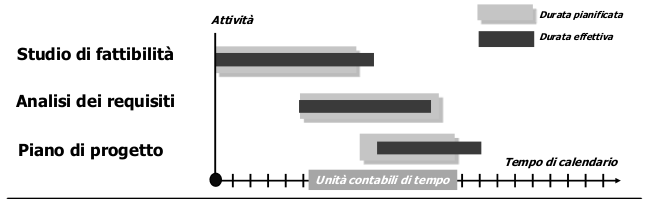
\includegraphics[width=0.5\textwidth]{img/gantt}		
			\caption{Esempio di diagramma di Gantt.}
		\end{figure} 
	
		\subsection{DIAGRAMMA DI PERT} \index{Diagramma di PERT} \label{pert}
		Questo tipo di diagramma (\textit{Programme Evaluation and Review Technique}) mostra le dipendenze temporali tra le varie attività al fine di ragionare sulle scadenze di progetto.
		
		\begin{figure}[H]
			\centering
			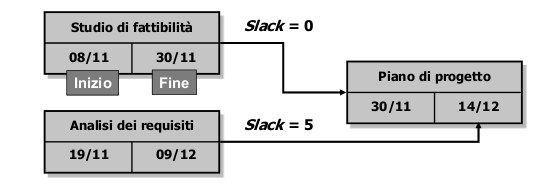
\includegraphics[width=0.5\textwidth]{img/pert}		
			\caption{Esempio di diagramma di PERT.}
		\end{figure} 
		
		Si parla qui di \textit{Slack time}: Si definisce "slack time" il periodo di tempo durante il quale un'attività può essere ritardata senza ritardare l'intero progetto di cui fa parte. Si calcola facendo la differenza tra l'ultima data disponibile per compiere l'attività e la prima data disponibile perché venga compiuta. Il cammino critico è la sequenza di attività ordinata con prodotto importante e dipendenze temporale strette.
		
		\subsection{DIMINISHING RETURNS}	\index{Diminishing returns}	\label{diminishingreturn}	%slide 7/34
		\textit{Ritorno in diminuzione}, c'è un certo punto in cui la curva dell'output decresce, ovvero andare avanti costa di più del beneficio che se ne trae. \\
		È il punto in cui i test non rilevano più gli errori.
		
		\subsection{DIVIDE ET IMPERA}	\index{Divide et Impera} \label{divideetimpera}		
		Se ho un prodotto fatto di parti riesco ad avere parallelismo nell'implementazione, in modo da andare \textit{n} volte più veloce.
		
		\subsection{DOCUMENTI}	\index{Documenti}	\label{documenti}	%!!
		I documenti adottano una strategia: come mi approccio al problema e come mitigo i rischi. La milestone è definita dalla strategia e applica il divide-et-impera (perchè divide tutto in problemi più piccoli). La strategia va SEMPRE FATTA ALL'INDIETRO. \\
		Tra i documenti da consegnare alla RR troviamo:
		\begin{itemize}
			\item \underline{\hyperref[piano]{PDP}}: quale strategia utilizzare, come nel tempo prepararci ad addomesticare i rischi, ecc;
			\item \underline{\hyperref[norme]{Norme di progetto}};
			\item ..
		\end{itemize} 
	
		\subsection{DRIVER}	\index{Driver}	\label{driver}
		È una componente attiva fittizia per pilotare il test e serve per eseguire su un'unità che non ha main.
	

	\newpage
	\flushright{\hyperref[index]{\color{black!65}{Ritorna all'indice}}}\flushleft
	\section{E} \label{sec:E}
	
		\subsection{ECONOMICITÀ} \index{Economicità} \label{economicita}
		L'insieme di \underline{\hyperref[efficienza]{efficienza}} ed \underline{\hyperref[efficacia]{efficacia}}.
		
		\subsection{EFFICACIA} \index{Efficacia} \label{efficacia}
		Capacità di produrre l'effetto e i risultati voluti. (In stretta correlazione a \underline{\hyperref[qualita]{qualità}}).
		
		\subsection{EFFICIENZA} \index{Efficienza} \label{efficienza}
		Capacità costante di rendimento e rispondenza per i propri fini senza sprecare risorse. Metrica di riferimento: \underline{\hyperref[produttivita]{produttività}}.
		
		\subsection{ENDEAVOR} \index{Endeavor} \label{endeavor}
		Atto costruttivo di fare (=tentativo/provare) comprende:
			\subsubsection{Work} \label{work}
			Attività e compiti da fare.
			\subsubsection{Team} \label{team}
			Perché collaborativo.
			\subsubsection{Way of working}	\label{way}
			Un team è un team soltanto se ha il suo modo di lavorare, cosa che sta alla base di tutto. Esso regola i \underline{\hyperref[processo]{processi}}.
		
		\subsection{ENGINEERING} \index{Engineering} \label{engineering}
		Applicazione pratica di principi scientifici e matematici. Ciò vuol dire che non \textit{crea} bensì \textit{attua} secondo la \underline{\hyperref[best]{best practice}}. Comporta inoltre responsabilità etiche e professionali.
		
		\subsection{ERROR}	\index{Error}	\label{error}
		È a monte della \textit{failure} e accade perché lo stato del sistema è sbagliato. Può essere meccanico, algoritmico o concettuale.
	
	

	\newpage
	\flushright{\hyperref[index]{\color{black!65}{Ritorna all'indice}}}\flushleft
	\section{F} \label{sec:F}
	
		\subsection{FAILURE}	\index{Failure}	\label{failure}	%V e V: analisi dinamica 20 dicembre
		L'effetto che vedo di un malfunzionamento. È un effetto finale che non mi aspettavo. \\
		In una versione gerarchica, più grande, un failure potrebbe generare un altro \textit{fault} che causa altri errori. %slide 6/34
	
		\subsection{FASE} \index{Fase} \label{fase}  
		Segmento contiguo di durata temporale che ha inizio e fine. É diviso a sua volta in altri segmenti. Può essere:
		\begin{itemize}
			\item di \underline{\hyperref[stato]{stato}};
			\item di transizione (stato che mi porta da x a y).
		\end{itemize}
	
		\subsection{FAULT}	\index{Fault}	\label{fault}
		È la ragione dell'\textit{error}, causa l'errore. Viene da un \textit{mistake} umano.
		
	
	

	\newpage
	\section{G} \label{sec:G}
		\subsection{GESTIONE DELLA CONFIGURAZIONE} \index{Gestione della configurazione} \label{gestioneconfigurazione}
		Processo di supporto implicato dall'\underline{\hyperref[analisideirequisiti]{Analisi dei requisiti}} che è un documento collaborativo in cui ognuno ha una determinata parte e non c'è confusione.

		\subsection{GESTIONE DEI CAMBIAMENTI} \index{Gestione dei cambiamenti} \label{gestionecambiamenti}
		Processo di supporto implicato dall'\underline{\hyperref[analisideirequisiti]{Analisi dei requisiti}} perchè l'analisi dei requisiti non è un'attività libera da vincoli. Ogni cambiamento deve avere un resoconto. \\
		Valuta la fattibilità tecnica e l'impatto sul progetto.

		\subsection{GESTIONE DEI REQUISITI}	\index{Gestione dei requisiti} \label{gestionerequisiti}
		Attività da svolgere per l'\underline{\hyperref[analisideirequisiti]{Analisi dei requisiti}}. Prevede l'identificazione e la \underline{\hyperref[classificazione]{classificazione}} dei \underline{\hyperref[requirements]{requisiti}}:
		\begin{itemize}
			\item Identificatore unico
			\item Numerazione sequenziale basata sulla struttura del documento
			\item Organizzazione secondo la coppia [\texttt{CATEGORIA}, \texttt{NUMERO}]
		\end{itemize}
		Avviene inoltre la \underline{\hyperref[gestionecambiamenti]{gestione dei cambiamenti}} e la \underline{\hyperref[tracciamento]{tracciabilità}} (\textit{requisiti} in rapporto a \textit{parti della specifica} in rapporto a \textit{componenti del sistema}).

		\subsection{GESTIONE DEI RISCHI} \index{Gestione dei rischi} \label{gestionerischi}
		Fa parte della \underline{\hyperref[gestioneprogetto]{gestione di progetto}}. Prevede:
			\begin{itemize}
				\item Identificazione dei rischi nel progetto, nel prodotto e nel mercato
				\item Analisi della probabilità di occorrenza e conseguenze possibili
				\item \underline{\hyperref[pianificazione]{Pianificazione}}, ovvero come evitare i rischi e mitigarne gli effetti
				\item Controllo, ovvero prestare continua attenzione tramite rilevazione di indicatori e raffinamento delle strategie
			\end{itemize}
		\begin{figure}[H]
			\centering
			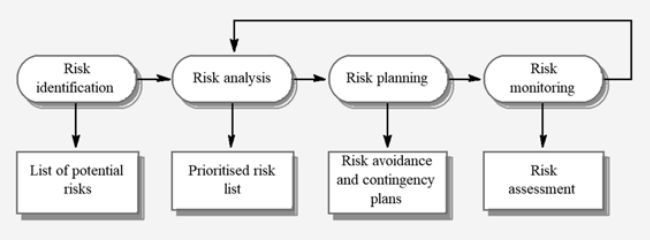
\includegraphics[width=0.8\textwidth]{img/rischi}
			\caption{Schema della gestione dei rischi.}
		\end{figure}



		\subsection{\emph{GESTIONE DI PROGETTO}} \index{Gestione di progetto} \label{gestioneprogetto}	%V.I.
		La gestione di progetto prevede:
			\begin{itemize}
				\item L'istanziazione di processi nel progetto secondo degli \underline{\hyperref[standard]{standard di processo}}
				\item La stima di costi e risorse necessarie tramite \underline{\hyperref[cocomo]{CoCoMo}}. I fattori di influenza per le stime sono:
				\begin{itemize}
					\item Dimensione del progetto
					\item Esperienza del dominio
					\item Familiarità con le tecnologie
					\item Produttività dell'ambiente di lavoro
					\item \underline{\hyperref[qualita]{Qualità}} attesa
				\end{itemize}
				\item \underline{\hyperref[pianificazione]{Pianificazione}} (partendo dall'obiettivo, quindi all'indietro, non dall'inizio) di attività con conseguente assegnamento alle varie persone
				\item Il controllo delle attività e la verifica dei risultati
			\end{itemize}
		In questo contesto ogni persona assume un certo \underline{\hyperref[ruoli]{ruolo}} e ad ogni ruolo viene assegnata un'attività (da notare che spesso molte risorse possono essere impegnate su più progetti). La gestione di progetto prevede anche la  \underline{\hyperref[gestionequalita]{Gestione di Qualità}} e un \underline{\hyperref[piano]{Piano di Progetto}}. \\
		I principali \textit{fattori di successo} di un progetto sono:
		\begin{itemize}
			\item Il coinvolgimento del cliente
			\item Il supporto della direzione esecutiva
			\item La definizione chiara dei requisiti
			\item Una pianificazione corretta
			\item Delle aspettative realistiche
			\item Un personale competente
		\end{itemize}
		Mentre i primi \textit{fattori di fallimento} sono:
		\begin{itemize}
			\item Dei requisiti incompleti
			\item Il mancato coinvolgimento del cliente
			\item La mancanza di risorse
			\item Delle aspettative non realistiche
			\item La mancanza di supporto  esecutivo
		\end{itemize}

		\subsection{GESTIONE DI QUALITÀ}  \index{Gestione di qualità} \label{gestionequalita}
		È una funzione di più recente introduzione aziendale. La \underline{\hyperref[qualita]{qualità}} riguarda qui sia i prodotti che i processi e interessa sia committente che la direzione aziendale. \\
		La garanzia di qualità produce confidenza, ma richiede l'applicazione rigorosa dei processi adottati e la loro \underline{\hyperref[manutenzione]{manutenzione}} migliorativa (ciclo di \underline{\hyperref[pdca]{PDCA}}).

	%\newpage
	\flushright{\hyperref[index]{\color{black!65}{Ritorna all'indice}}}\flushleft
	\section{H} \label{sec:H}
	
	

	\newpage
	\section{I} \label{sec:I}


		\subsection{IMPLEMENTATION} \index{Implementation} \label{implementation}
		Termine inglese per \textit{codifica}. Si tratta di realizzare concretamente quello che nel progetto è stato precedentemente ideato.


		\subsection{INCAPSULAMENTO} \index{Incapsulamento} \label{incapsulamento}
		Un meccanismo del linguaggio di programmazione atto a limitare l'accesso diretto agli elementi dell'oggetto.


		\subsection{INCREMENTO} \index{Incremento} \label{incremento}
		Modo di avvicinarsi sempre di più a destinazione ``aggiungendo qualcosa che mi porta verso la meta''.


		\subsection{INSPECTION}	\index{Inspection}	\label{inspection}
		È un metodo pratico di lettura come \underline{\hyperref[walkthrough]{Walkthrough}}. Ha come obiettivo rilevare la presenza di difetti eseguendo una lettura mirata. Chi la fa sono \underline{\hyperref[verificatore]{Verificatori}} distinti dai \underline{\hyperref[programmatore]{Programmatori}} e la strategia che viene adottata si focalizza sulla ricerca con presupposti. \\
		In ogni fase delle attività svolte deve avvenire la documentazione:
		\begin{enumerate}
			\item Pianificazione
			\item Definizione lista di controllo
			\item Lettura
			\item Correzione dei difetti
		\end{enumerate}
		\textbf{Differenze}: Walkthrough richiede maggiore attenzione ed è più collaborativo, mentre Inspection è più rapido e basato su presupposti.


		\subsection{INTEGRAZIONE CONTINUA} \index{Integrazione continua} \label{integrazione}
		In modo dimostrabile \underline{\hyperref[incremento]{Incremento}} e non itero. Vado quindi verso la meta e ogni passo che eseguo ha un valore.


		\subsection{ITERAZIONE} \index{Iterazione} \label{iterazione}
		Procedere per raffinamenti o rivisitazioni ``aggiungendo o togliendo qualcosa che mi fa quindi avanzare o retrocedere''.

	\newpage
	\section{J} \label{sec:J}

		\subsection{JOINT REVIEW PROCESS} \index{Joint Review Process} \label{joint}
		Tratta di revisioni di monitoraggio.
		Si tratta di una revisione \textbf{interna} (in particolare  \underline{\hyperref[RP]{RP}} e \underline{\hyperref[RQ]{RQ}}).

	%\newpage
	\section{K} \label{sec:K}
	
	

	\newpage
	\flushright{\hyperref[index]{\color{black!65}{Ritorna all'indice}}}\flushleft
	\section{L} \label{sec:L}
	
		\subsection{LOGGER}	\index{Logger}	\label{logger}
		Componente non intrusivo di registrazione dei dati di esecuzione per analisi dei risultati, quale per esempio un \textit{bot} (così l'umano non deve fare da sè il test).
	
	

	\newpage
	\section{M} \label{sec:M} 
	
		\subsection{MANUALI}	\index{Manuali} \label{manuali}
		Uno dei prodotti che racconta il prodotto all'utente.
		
		\subsection{MANUALE DELLA QUALITÀ} \index{Manuale della qualità} \label{manualequalita} % (slide 10) Set Lezione del 4/12 - Qualità di processo
		Il documento che definisce il sistema di gestione della qualità di un’organizzazione. Ha una visione ad alto livello. Si integra con i processi e le procedure aziendali e fissa gli obiettivi di qualità aziendali e le strategie per perseguirli.
	
		\subsection{MANUTENZIONE} \index{Manutenzione} \label{manutenzione}
		Complesso delle operazioni necessarie a conservare la conveniente funzionalità ed \underline{\hyperref[efficienza]{efficienza}}. Può essere:
			\begin{itemize}
				\item \textbf{correttiva} = rimozione di difetti;
				\item \textbf{adattativa} = raffinamento dei \underline{\hyperref[requirements]{requisiti}};
				\item \textbf{evolutiva} = evoluzione del sistema;
			\end{itemize}
		Dato che bisogna avere memoria di quello che ha funzionato e quello che funziona ora, possiamo dire che un prodotto sotto manutenzione ha una storia, ed essa va gestita con \underline{\hyperref[controllodiversione]{controllo di versione}}.
			
		\subsection{MATURITÀ} \index{Maturità} \label{maturita} %(slide 14) Set Lezione del 4/12 - Qualità di processo
		Misura la \underline{\hyperref[qualita]{qualità}} dei \underline{\hyperref[processo]{processi}}, ovvero misura quanto (e quanto bene) l’azienda è governata dal suo sistema di processi. È quindi caratteristica di un insieme di processi e rappresenta il risultato delle \textit{\underline{\hyperref[capability]{capability}}} dei processi considerati.
		\begin{figure}[H]
			\centering
			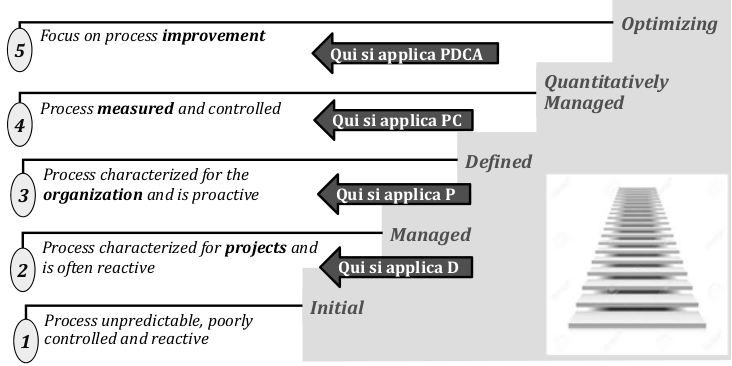
\includegraphics[width=0.9\textwidth]{img/maturity}		
			\caption{I 5 livelli di maturità per la qualità di processo.}
		\end{figure} 
		I livelli di maturità di \underline{\hyperref[cmmi]{CMMI}} mi aiutano a capire con quale intelligenza agisco.\\
		La maturità di prdotto valuta il grado di evoluzione del prodotto: quanto migliora in seguito alle prove, quanto diminuisce la densità dei difetti, quanto può costare la scoperta del prossimo difetto.
		
		\subsection{METRICA} \index{Metrica} \label{metrica} 
		Integrale degli usi o utenti nel tempo.\\
	
		La \textit{Metrica Software} comprende:
			\begin{itemize}
				\item \textit{SLOC} (= Source Lines Of Code): conta le linee, è quindi oggettivamente misurabile e dà limiti;
				\item \textit{Effort}: risorse umane misurate come giorni/persona.
				\item \textit{Testo}: perché il testo è facilmente offuscabile, quindi si usa "l'indice di nebbia"/leggibilità. 
			\end{itemize}
		Dà il modo di classificare attributi di processo e ci aiuta a ragionare a monte del problema e non a valle. In questo modo si possono predire gli attributi che arriveranno (capire prima se il prodotto farà schifo). L'obiettivo è quello di identificare anomalie \textit{"the sooner the better"}. \\
		Associate alla \underline{\hyperref[qualita]{Qualità del Software}} c'è l'idea di \textit{assunzioni} sulle metriche: nostro modo di pensare al problema. Attenzione perché non sempre si può misurare ciò che vogliamo. Ci interessa misurare ciò che è tracciabile di quello che vogliamo sapere (esempio dell'analisi del sangue: voglio sapere una cosa di alto livello non misurabile, tramite dati del mio sangue che sono misurabili). Importanti attributi sono: manutenibilità, affidabilità, \underline{\hyperref[portabilita]{portabilità}} e usabilità.
		
		\subsection{MISTAKE}	\index{Mistake}	\label{mistake}
		Ci siamo sbagliati noi nel produrre qualcosa che se utilizzato  nel SW, causerà errore. Questo è quindi a monte di tutto (vedi problemi nei \underline{\hyperref[test]{test}}).		 
		
		\subsection{MOCK}	\index{Mock}	\label{mock}
		I \textit{mock object} (simulati o mock object) sono degli oggetti simulati che riproducono il comportamento degli oggetti reali in modo controllato. Nella programmazione ad oggetti, un programmatore crea un oggetto mock per testare il comportamento di altri oggetti, reali, ma legati ad un oggetto inaccessibile o non implementato. Allora quest'ultimo verrà sostituito da un mock.
		
		\subsection{MODELLI DI SVILUPPO} \index{Modelli di sviluppo} \label{modelli}
		Il modello è una costruzione astratta che fa capire qual è il problema e dà strumenti per risolverlo. È un riferimento ideale ad una cosa concreta, quindi astrazione non eseguibile, ma che mi definisce le proprietà. Date le diverse transizioni previste tra gli stati di un ciclo di vita e diverse regole di attivazione, esistono diversi tipi di modelli.
		%Flipped Classroom 6 dicembre
		I modelli, per essere tali, sono tutti "buoni". Semplicemente alcuni sono più adatti a certe esigenze rispetto ad altri.
		\begin{itemize}
			\item \textbf{A cosa serve}:
			Tre cose hanno fortissima influenza sulla scelta da fare:
			\begin{itemize}
				\item obiettivi;
				\item rischi;
				\item vincoli;
			\end{itemize}
			Serve a perseguire gli obiettivi cercando di rispettare i vincoli e mitigando i rischi.
			\item \textbf{Di cosa è fatto}:
			Il modello di sviluppo è legato al progetto da portare a termine e il progetto determina i processi. Quindi i processi hanno a che vedere con il modello di sviluppo. C'è un importante ordine di attività. Chi decide quali sono i \textit{gate} (momento in cui si termina un'attività e si passa a quella successiva) siamo noi, ovvero il fornitore, in base a quali obiettivi raggiungere nel tempo. Le milestone coincidono con i nostri gate. Le milestone c'entrano infatti sia con obiettivi, che con rischi e vincoli. \\
			Per dare elementi di mitigazione ai rischi ho la \underline{\hyperref[technologybaseline]{Technology Baseline}}. [Quante milestone ho lo decide il fornitore. La baseline sono le evidenze che porto per aprire i gate. Prima vengono le milestone e poi le baseline.] \\
			Il \underline{\hyperref[semat]{SEMAT}} mi dà l'essenza che sta alla radice di ogni modello di sviluppo. Dal SEMAT riesco a capire quali milestone adottare nel mio piano. E tra quelle che posso scegliere, le milestone che scelgo devono essere una confluenza di quelle più specializzate (ricordare le cards). Ho tante baseline quanti "lucchetti"(milestone) da aprire.
			\item \textbf{Come lo si attiva}: individuando le attività riconoscibili dalle baseline che ho scelto mettendole nel tempo disponibile e assegnandole.
		\end{itemize}	
		
			\subsubsection{Sequenziale (o a cascata)} \index{Modello sequenziale} \label{msequenziale}
			\textbf{In breve}: ha rigide fasi sequenziali. \\
			 Tutto deve essere ripetibile (quindi anche migliorabile) e lineare (successioni di \underline{\hyperref[fase]{fasi}}), ma non ammette un ritorno a fasi precedenti. Adotta quindi una strategia in cui si continua o al più ci si ferma. Si prosegue solo se l'azione viene considerata buona (quindi documentata prima). I suoi prodotti sono principalmente \textit{documenti}. Ogni fase è caratterizzata da pre e post condizioni (di ingresso le prime e di uscita le seconde) e viene definita in termini di responsabilità e ruoli coinvolti. Dato che le fasi sono durate temporali, devono essere distinte e non sovrapposte nel tempo, dato che presentano delle dipendenze causali tra loro. Lo schema per il modello a cascata prevede in ordine: \underline{\hyperref[analisideirequisiti]{Analisi}} - \underline{\hyperref[progettazione]{Progettazione}} - \underline{\hyperref[realizzazione]{Realizzazione}} - \underline{\hyperref[manutenzione]{Manutenzione}}.  \\
			 \textbf{Difetto}: è totalmente rigido quindi ha bisogno di correttivi (come i \underline{\hyperref[prototipo]{prototipi}}).
			 
			 \begin{figure}[H]
			 	\centering
			 	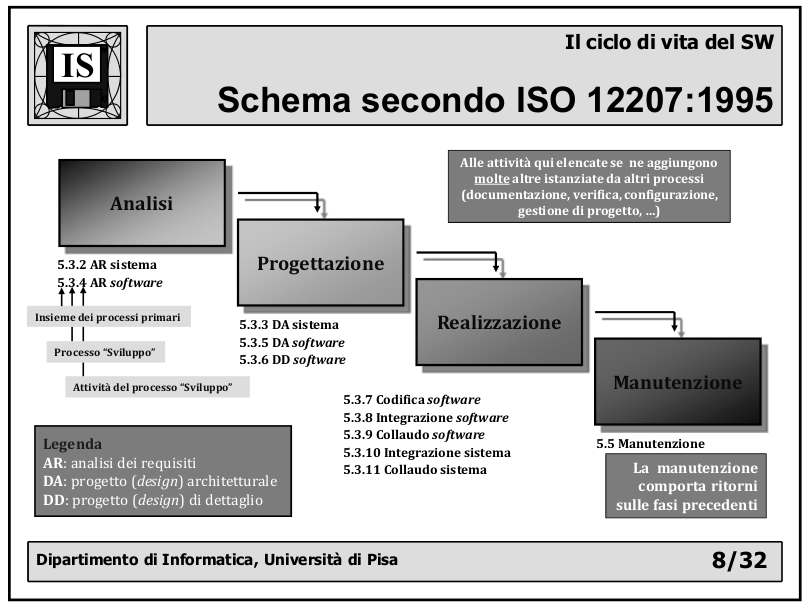
\includegraphics[width=0.8\textwidth]{img/cascata}		
			 	\caption{Schema del modello a cascata secondo lo \underline{\hyperref[standard]{standard}} ISO 12207.}
			 \end{figure} 
			
			\subsubsection{Incrementale} \index{Modello incrementale} \label{mincrementale}
			\textbf{In breve}: realizzazione in più passi, prevede rilasci multipli e successivi, ciascuno realizza un incremento di funzionalità. \\
			Dato che spesso non conviene posticipare l'integrazione di tutte le parti del sistema, risulta migliore l'\underline{\hyperref[integrazione]{integrazione continua}} di piccole parti. Sceglie un ordine di sviluppo che prepari il passaggio successivo motivo per cui ci vuole un modo strategico per capire come muoversi. I primi incrementi possono essere frutto di prototipazione,
			aiutando a fissare meglio i requisiti per gli incrementi successivi, ma i primi incrementi puntano a soddisfare i requisiti più importanti sul piano strategico così essi diventano presto chiari e stabili e quelli meno importanti si possono armonizzare al sistema. Ogni incremento riduce quindi il rischio di fallimento. Analisi e progettazione architetturale non vengono ripetute, dato che l'architettura del sistema è ben identificata e fissata dall'inizio, invece la realizzazione è incrementale (al momento della validazione può avvenire un ritorno).
			
			\begin{figure}[H]
				\centering
				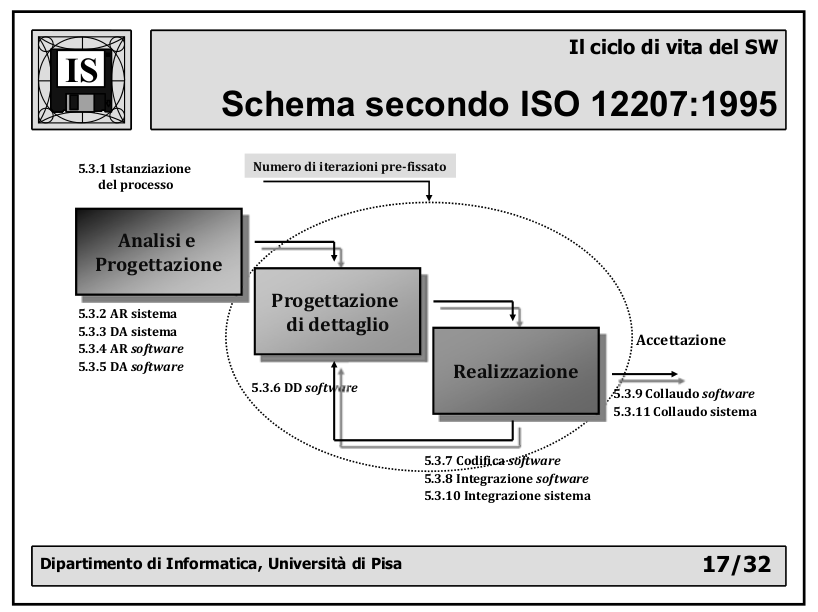
\includegraphics[width=0.8\textwidth]{img/incrementale}		
				\caption{Schema del modello incrementale secondo lo \underline{\hyperref[standard]{standard}} ISO 12207.}
			\end{figure} 
			
			\subsubsection{Iterativo} \index{Modello iterativo} \label{miterativo}
			\textbf{In breve}: ha ripetute iterazioni interne. \\
			Questo tipo di modello è applicabile a qualunque modello di ciclo di vita; consente infatti maggior capacità di adattamento. Il problema è che può andare incontro al rischio di non convergenza perché ogni iterazione comporta un ritorno all'indietro nella direzione opposta all'avanzamento del tempo. In generale conviene quindi decomporre la realizzazione del sistema in parti più piccole trattando prima le parti più critiche (magari quelle i cui requisiti vanno maggiormente chiariti). 
			
			\subsubsection{A evoluzioni successive} \index{Modello a evoluzioni successive}
			\textbf{In breve}: comporta il riattraversamento di più stati di ciclo di vita. \\ 
			 \underline{\hyperref[prodotto]{Prodotto}} che evolve come conseguenza di una \underline{\hyperref[manutenzione]{manutenzione}}. Aiuta a rispondere a bisogni non inizialmente preventivabili. Inizialmente viene fatta un'analisi preliminare che identifica i requisiti e definisce l'architettura di massima e pianifica i passi di analisi. Dopodiché avviene l'analisi e realizzazione di una singola evoluzione (per raffinamento dell'analisi iniziale o per progettazione-codifica-prove-integrazione). Infine c'è il rilascio di versioni che man mano saranno sempre più complete. Ogni fase ammette iterazioni multiple e parallele.
			 
			 \begin{figure}[H]
			 	\centering
			 	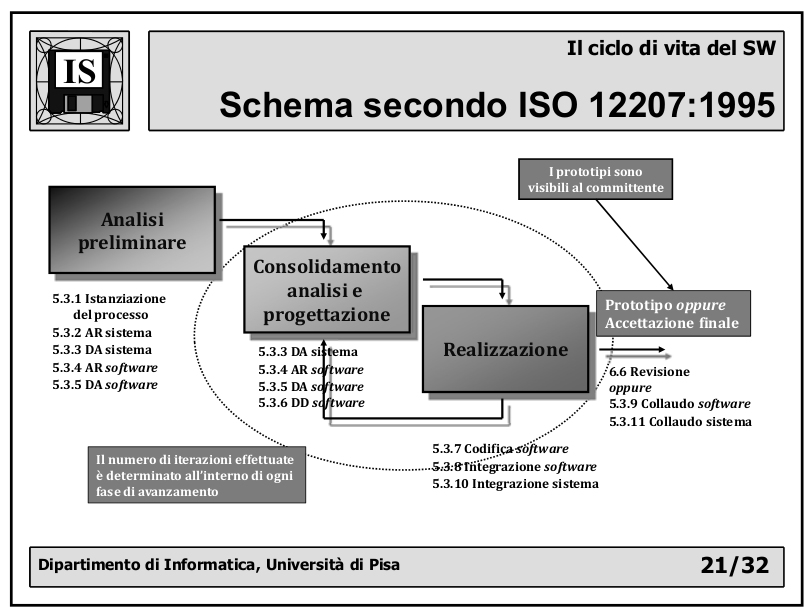
\includegraphics[width=0.8\textwidth]{img/evoluzione}		
			 	\caption{Schema del modello evolutivo secondo lo \underline{\hyperref[standard]{standard}} ISO 12207.}
			 \end{figure} 	
			
			\subsubsection{Per componenti} \index{Modello per componenti}
			\textbf{In breve}: è orientato a massimizzare il riuso di software. \\
			 Decomposto in parti già esistenti e funzionanti, riusabili. L'analisi dei requisiti viene in seguito rivisitata in base alle possibilità di riuso.
			
			\begin{figure}[H]
				\centering
				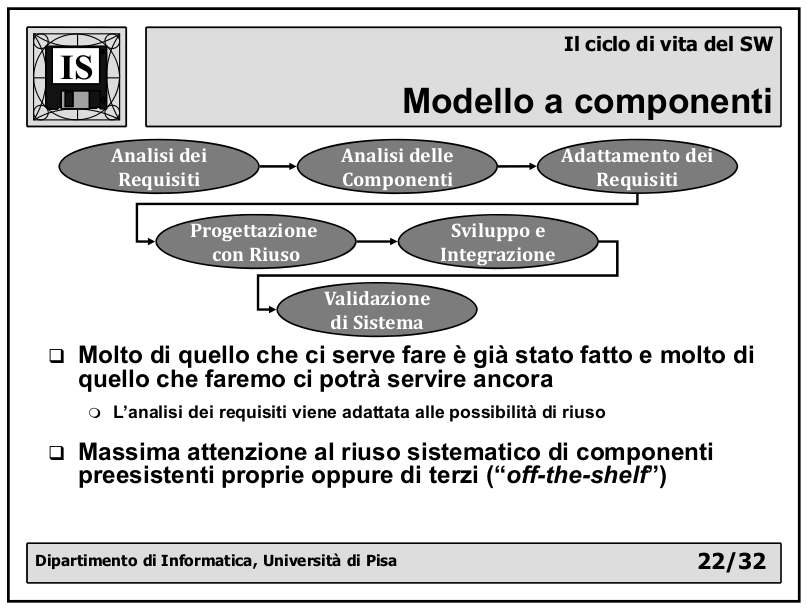
\includegraphics[width=0.8\textwidth]{img/acomponenti}		
				\caption{Schema del modello a componenti secondo lo \underline{\hyperref[standard]{standard}} ISO 12207.}
			\end{figure} 
		
			\paragraph{Il riuso}
			Dal Sommerville sappiamo del \textbf{riuso} che: \\
			Le unità software riusate possono avere diversa dimensione, per esempio:
			\begin{itemize}
				\item \textbf{System reuse}: un intero sistema (che può essere composto da più applicazioni) può essere riusato come parte di un sistema di tanti sistemi
				\item \textbf{Application reuse}: un'applicazione può essere riusata incorporandola in altri sistemi senza fare cambiamenti, oppure configurando l'applicazione per diversi customers
				\item \textbf{Component reuse}: componenti di un'applicazione (da sotto-sistemi a singoli oggetti) possono essere riusate. Per esempio, un sistema di sviluppo che fa pattern-matching, che fa parte di in un sistema di text-processing, può essere riusato in un sistema di gestione di database. Le componenti possono risiedere in un cloud o in server privati e possono essere accessibili tramite Application Programming Interface (API). 
				\item \textbf{Object and function reuse}: componenti software che implementano una singola funzione o una classe oggetto possono essere riusate. Molte librerie di funzioni e classi sono liberamente disponibili. Si riusano classi e funzioni in queste librerie collegandole con lo sviluppo di nuovo codice.
			\end{itemize}	
			A volte i sistemi o componenti sono così specifici che è molto costoso modificarli per una nuova situazione. Quindi, più che riusare il codice, è possibile riusare le idee che stanno alla base del software. Questo è chiamato \textbf{concept reuse} e tratta per esempio di riusare un way of working o un algoritmo e approcci quali i design patterns. \\
			I benefici del riuso sono:
			\begin{itemize}
				\item Costo complessivo di sviluppo più basso, perché meno componenti software devono essere progettate, implementate e validate
				\item Sviluppo accelerato
				\item Aumento di affidabilità, perchè software che è stato provato e testato in altri sistemi funzionanti è più affidabile di un nuovo software. I suoi difetti di progettazione e implementazione dovrebbero già esser stati trovati e sistemati.
				\item  Ridotto rischio di processo, vero specialmente per grandi componenti software riusate come sottosistemi. È un fattore importante per il Project Manager perché riduce il margine di errore nella stima dei costi di un progetto.
				\item Conformità con gli standard, perché alcuni standard, come gli interface standard, possono essere implementati come set di componenti riusabili
			\end{itemize}
			Ci sono però anche delle difficoltà legate al riuso come:
			\begin{itemize}
				\item Costo associato al capire se una componente è adatta al riuso per una particolare situazione o meno. È un costo aggiuntivo che potrebbe essere così elevato che potrebbe non abbassare il costo complessivo di sviluppo
				\item Creare, mantenere e usare la componente di una libreria, perché può essere oneroso
				\item Maggiori costi di manutenzione, perché se il codice sorgente della componente riusate non è disponibile, gli elementi riusati del sistema potrebbero diventare incompatibili con i cambiamenti fatti al sistema.
				\item Mancanza di strumenti di supporto, perché alcuni tools non supportano lo sviluppo con riuso.
				\item "Not-invented-here" syndrome, ovvero il fatto che alcuni software engineers preferiscono riscrivere componenti perchè credono di poterle migliorare
			\end{itemize}
			Fattori da considerare quando si sta pianificando il riuso:
			\begin{itemize}
				\item \textbf{The development schedule for the software}: se il software deve essere sviluppato velocemente, bisognerebbe riusare completamente un sistema piuttosto che una componente singola.
				\item \textbf{The expected software lifetime}: se si pensa ad un sistema con ciclo di vita lungo, bisognerebbe concentrarsi sulla manutenibilità del sistema. In questo caso si mira a riusare sistemi e componenti open-source più sicuri.
				\item \textbf{The background, skills and experience of the development team}: la cosa migliore è focalizzarsi nel riuso di aree in cui il team ha esperienza
				\item \textbf{The criticality of the software and its non-functional requirements}: per un sistema che deve essere certificato da un regolatore esterno, bisognerebbe creare una parte di sicurezza, ma questo è difficile se non si ha accesso al codice sorgente. Per esempio, se il software ha dei requisiti stringenti potrebbe risultare impossibile usare strategie quali il model-driven engineering (MDE).
				\item \textbf{The application domain}: in molti domini applicativi, come sistemi industriali e d'informazione medica, ci sono prodotti generici che possono essere riusati in una situazione locale. Qui fare riuso è spesso conveniente. 
				\item \textbf{The platform on which the system will run}: come i .NET sono specifici delle piattaforme Microsoft, esistono sistemi di applicazioni generici che sono specifici di una certa piattaforma. Si è quindi in grado di riusare solo se il nostro sistema è progettato per la stessa piattaforma.  
			\end{itemize}
		
		 	Per quel che riguarda i framework, Schimdt sostiene che il framework è: \textit{an integrated set of software artifacts (such as classes, objects and components) that collaborate to provide a reusable architecture for a family of related applications}. I frameworks forniscono supporto per caratteristiche generiche che possono essere usate in tutte le applicazioni di tipo simile. \\
		 	Quando una compagnia deve supportare un numero di sistemi simili ma non identici, uno degli approcci di riuso più efficaci è creare una \textit{software product line}. Una \textit{software product line} è un set di applicazioni con un'architettura comune e componenti condivise in cui ogni applicazione è specializzata per riflettere specifici requisiti del cliente.  Generalmente un'applicazione base include:
		 	\begin{itemize}
		 		\item \textbf{Core components}: forniscono un'infrastruttura di supporto e di solito non vengono modificate quando viene sviluppata una nuova istanza della \textit{software product line}.
		 		\item \textbf{Configurable application components}: possono essere modificate e configurate per specializzare una nuova applicazione.
		 		\item \textbf{Specialized application components}: specifiche del dominio, alcune o tutte possono essere rimpiazzare quando una nuova istanza della \textit{software product line} viene creata.
		 	\end{itemize}
	 	 	
	 	 	\paragraph{CBSE}
	 	 	Le componenti sono ad un livello di astrazione più alto degli oggetti e sono definite dalle loro interfacce. Sono solitamente più grandi degli oggetti singoli e tutti i dettagli implementativi sono nascosti alle altre componenti. \\
	 		\textit{Component-based software engineering} è il processo di definizione, implementazione e integrazione o composizione di queste componenti scarsamente accoppiate e indipendenti nei sistemi.  \\
	 		Le caratteristiche essenziali un una componente usate nel CBSE (\textit{Component-based software engineering}):
	 		\begin{itemize}
	 			\item \textbf{Composable}
	 			\item \textbf{Deployable}
	 			\item \textbf{Documented}
	 			\item \textbf{Independent}
	 			\item \textbf{Standardized}
	 		\end{itemize}
 			Un modo utile di vedere una componente è vederla come un fornitore di uno o più servizi:
 			\begin{itemize}
 				\item La \textbf{componente} è un'entità eseguibile indipendente che viene definita dalla sua interfaccia. Non c'è bisogno di saperne il codice sorgente per usarla.
 				\item I \textit{servizi} offerti da una componente sono resi disponibili attraverso un'interfaccia e tutte le interazioni avvengono tramite quell'interfaccia. L'interfaccia della componente è espressa in termini di operazioni parametrizzate e il suo stato interno non è mai esposto.
 			\end{itemize}
 			Di base tutte le componenti hanno due interfacce collegate:
 			
 			\begin{figure}[H]
 				\centering
 				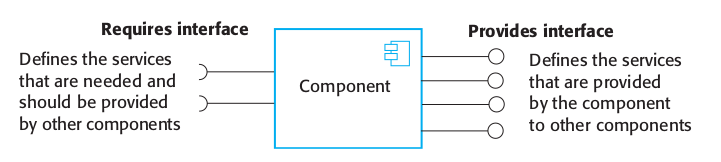
\includegraphics[width=0.8\textwidth]{img/interfaces}		
 				\caption{Interfacce di una componente.}
 			\end{figure} 
 			
 			\begin{itemize}
 			 	\item La \textit{requires interface} specifica i servizi che le altre componenti del sistema devono fornire affinchè la componente funzioni correttamente. Se questi servizi non sono disponibili, la componente non funzionerà.
 			 	\item La \textit{provides interface} definisce i servizi forniti dalla componente. Quest'interfaccia è la componente API.
 			\end{itemize} 
 		
 			\paragraph{Component models}
 			Un \textit{component model} è una definizione di standard per l'implementazione, la documentazione e il deployment di componenti. Questi standard sono per gli sviluppatori delle componenti per assicurare che le componenti siano interoperabili. Per \textit{service components} il più importante modello a componenti è il Web Service model, mentre per le \textit{embedded components} sono ampiamenti usati i modelli Enterprise Java Beans(EJB) e Microsoft's .NET.
 			
 			\begin{figure}[H]
 				\centering
 				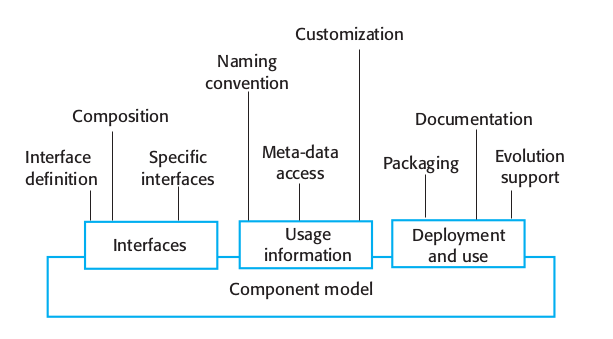
\includegraphics[width=0.8\textwidth]{img/componentmodel}		
 				\caption{Elementi base di un component model.}
 			\end{figure} 
 		
 			\paragraph{CBSE processes}
 			I processi CBSE sono processi software che supportano la \textit{Component-Based Software Engineering}. Ne esistono di due tipi:
 			\begin{itemize}
 				\item \textbf{Development for reuse}: processo mirante allo sviluppo di componenti o servizi che saranno riusati in altre applicazioni. Generalmente coinvolge componenti generiche già esistenti.
 				\item \textbf{Development with reuse}: processo che sviluppa nuove applicazioni usando componenti e servizi esistenti.
 			\end{itemize}
 		
			
			\subsubsection{Agile} \index{Modello agile}
			\textbf{In breve}: è altamente dinamico ed è fatto di brevi ciclo iterativi e incrementali. \\
			Basato su principi fortemente di reazione che sono:
				\begin{enumerate}
			 		\item \textit{Individuals and interactions over processes and tools}: l’eccessiva rigidità ostacola l’emergere del valore;
			 		\item \textit{Working sofware over comprehensive documentation}: la documentazione non sempre corrisponde a SW funzionante
			 		\item \textit{Customer collaboration over contract negotiation}: l’interazione con gli stakeholder va incentivata;
			 		\item \textit{Responding to change over following a plan}: la capacità di adattamento al cambiare delle situazioni;
			 	\end{enumerate}
		 	Si basa sull'idea di \textit{user story}, ovvero una funzionalità che è significativa per l'utente e che vuole nella realizzazione del software richiesto. Ogni \textit{user story} è definita un documento che descrive il problema, una sintesi delle conversazioni di discussione del problema con gli \underline{\hyperref[stakeholder]{stakeholder}} e la strategia da adottare per soddisfare il problema. Si prosegue suddividendo il lavoro in piccoli  \underline{\hyperref[incremento]{incrementi}} (che possono essere sviluppati anche indipendentemente) sviluppati in modo continuo e sequenziale dall'analisi all'integrazione. Gli \textit{obiettivi strategici} sono poter dimostrare costantemente al cliente quanto fatto e che l'intero  \underline{\hyperref[prodotto]{prodotto SW}} sia ben integrato e verificato. 
		 	[NB: Non é molto buono. É assente la documentazione quindi é più un costo che un valore]
			
			\subsection{SCRUM}	\index{Modello SCRUM}	\label{scrum}
			\textbf{In breve}: è un tipo di Modello Agile ["mischia di rugby"]. \\
			È costituito da:
				\begin{itemize}
					\item \textbf{Product \underline{\hyperref[backlog]{backlog}}}: requisiti e funzionalità del prodotto;
					\item \textbf{Sprint}: fase operativa di sviluppo;
					\item \textbf{Sprint \underline{\hyperref[backlog]{backlog}}}: insieme di storie del prossimo sprint;
					\item \textbf{Sprint Planning}: pianificazione dello sprint;
					\item \textbf{Daily Scrum}: controllo giornaliero dell'avanzamento;
					\item \textbf{Sprint Review}: controllo prodotti dello sprint;
					\item \textbf{Sprint Retrospective}: controllo \underline{\hyperref[qualita]{qualità}} sullo sprint;
				\end{itemize}
			
			\subsubsection{A spirale} \index{Modello a spirale}
			(Complicato, non lo trattiamo). Va da un problema piccolo ad uno sempre più grande. Pensato per attività che non hanno una \underline{\hyperref[best]{best practice}} ben nota.
			
						
			
		\subsection{MODULI}	\index{Moduli}	\label{moduli}
		La più piccola entità progettuale che sia utile rappresentare.	
	
	

	\newpage
	\section{N} \label{sec:N}
	
		\subsection{NORME DI PROGETTO}	\index{Norme di Progetto} \label{norme}
		È un documento \textbf{interno} che serve a istituire un way of woking (come ci impegniamo a lavorare) per noi incrementale. Deve essere un documento leggero cioè facile da consultare e da modificare.
		Le norme di progetto includono come programmare; nello specifico il processo di sviluppo contiene le norme di codifica.
		
		

	\newpage
	\section{O} \label{sec:O}
	
		\subsection{OPPORTUNITY} \index{Oppurtunity} \label{opportunity}
		Bisogno di un cliente che vale la pena di soddisfare.
	
		\subsection{ORACOLO}	\index{Oracolo}	\label{oracolo}	%V e V: analisi dinamica 20 dicembre
		È un elemento di una \underline{\hyperref[testsuite]{prova}}. \\
		Colui che risponde a tutti i dubbi e domande. È un metodo per generare a priori i risultati attesi e per convalidare i risultati ottenuti nella prova.
		Generalmente viene applicato da agenti automatici, per velocizzare la convalida e renderla ``oggettiva''. \\
		Si producono oracoli sulla base di specifiche funzionali con prove semplici tramite l'uso di componenti di terze indipendenti.
		
	

	\newpage
	\section{P} \label{sec:P}

		\subsection{PPP}	\index{PPP}	\label{3p}
		Stanno per: \textit{Product}, \textit{Process}, \textit{Progression in learning} (e Incrementalmente). Sono i 3 (4) punti di avanzamento chiave del progetto. Le 3P sono la \textit{capstone}(=parte finale di una struttura) project.
		
		\subsection{PIANIFICAZIONE} \index{Pianificazione} \label{pianificazione}
		Definisce delle attività al fine di pianificarne lo svolgimento e controllarne l’attuazione, avere una base su cui gestire l’allocazione delle risorse e per stimare e controllare scadenze e costi. Per la pianificazione vengono utilizzati degli \textit{strumenti} quali: \underline{\hyperref[gantt]{Diagramma di Gantt}}, \underline{\hyperref[pert]{PERT}} e \underline{\hyperref[wbs]{WBS}}. \\		
		In breve: chi fa cosa - quando - in quanto tempo - quanto costa. 
	
		\subsection{PIANO DI PROGETTO} \index{Piano di progetto} \label{piano}
		Il piano di progetto (o \textit{PdP}) sostanzialmente è un documento ufficiale, soggetto ad approvazioni, con il quale si descrivono gli obiettivi di progetto e gli elementi necessari per il loro raggiungimento. Si vedono le risorse disponibili e le loro assegnazioni alle attività con scansione delle attività nel tempo. L'attività più importante è l'analisi dei rischi. \\
		Principalmente è scomposto in:
			\begin{itemize}
				\item Pianificazione(preventiva)
					\begin{itemize}
						\item team;
						\item \underline{\hyperref[analisirischi]{analisi dei rischi}};
					\end{itemize}
				\item \underline{\hyperref[consuntivo]{Consuntivazione}}: è lo specchio della pianificazione. Fa una valutazione retrospettiva;
			\end{itemize}
		Tipicamente la struttura del PdP è composta da:
			\begin{itemize}
				\item Introduzione (scopo e struttura);
				\item Organizzazione del progetto;
				\item \underline{\hyperref[analisirischi]{Analisi dei rischi}};
				\item Risorse disponibili (tempo e persone);
				\item Suddivisione del lavoro (work breakdown);
				\item Calendario delle attività (project schedule);
				\item Meccanismo di controllo e di rendicontazione;
			\end{itemize}
		È da tenere presente che ci sono anche dei rischi di progetto, quali sforamento di costi o tempi, che derivano da fonti come tecnologie di lavoro e produzione, rapporti interpersonali, organizzazione del lavoro, rapporti con gli stakeholder e appunto tempi e costi. Per questo ci vuole una \underline{\hyperref[gestionerischi]{Gestione dei rischi}}. 
		
		%Quali contenuti:
		%Quale struttura:
		
		\subsection{PIANO DI QUALIFICA}	\index{Piano di Qualifica}	\label{pianoqualifica}
		Definisce le strategie di \underline{\hyperref[verificare]{verifica}} e \underline{\hyperref[validare]{validazione}} (metodi, tecniche, procedure, strumenti e tempi). Per ogni passo fatto in analisi o altro, preparare i test e fare il tracciamento per non perdere nulla, per dare qualità (consultare \underline{\hyperref[V]{modello a V}}); questo documento specifica quali e quante prove effettuare. Anche questo documento, come le \underline{\hyperref[norme]{Norme}}, è incrementale. \\
		Si parla qui di metriche e obiettivi di "oggi" (ad esempio requisiti, fluttuazione requisiti). \\
		\textbf{N.B:} le metriche vanno inserite nelle Norme (vedere correzione Breaking Bug) mentre gli obiettivi nel PdQ.
		
		\subsection{PIANO DI QUALITÀ}	\index{Piano di Qualità}	\label{pianoqualita} %slide 8/22 Set Qualità del software
		Attività del sistema qualità mirante a fissare gli obiettivi di \underline{\hyperref[qualita]{qualità}}, e i processi e le risorse necessarie per conseguirli. \\
		Stabilisce qual è il modo in cui noi perseguiamo la qualità. Si fissano le politiche aziendali e si determinano gli obiettivo di qualità del singolo progetto.
		
		\subsection{PORTABILITÀ}	\index{Portabilità}	\label{portabilita}
		Un prodotto che ha la proprietà di adattarsi ad altri dispositivi.
		  		 
		\subsection{PREVENTIVO} \index{Preventivo} \label{preventivo}
		Stima iniziale dei costi necessari alla realizzazione di un \underline{\hyperref[progetto]{progetto}}. (PAF = preventivo a finire, da attuarsi in corso d'opera perché diventa sempre più preciso).
	
		\subsection{PRINCIPIO DEL MIGLIORAMENTO CONTINUO} \index{Principio del miglioramento continuo} \label{miglioramentocontinuo}
		Identifica specifici obiettivi di miglioramento, li esegue, ne verifica l'esito e infine agisce sulle conseguenze (per esempio, se considerato buono, lo tiene nello standard).
		
		\subsection{PROBLEM RESOLUTION}	\index{Problem solution}	\label{problemsolution}
		Avere un metodo molto chiaro non violabile per la soluzione di problemi. È di \underline{\hyperref[12207]{ISO 12207}}. \\
		È fatto di una strategia nota (il nostro way of working). In essa tutti i problemi sorti sono stati registrati e ogni problema va studiato individualmente decidendo quali soluzioni sono accettabili. Viene in seguito realizzata la soluzione scelta e verificato l'esito della correzione. % slide 10/22
		È comunque un'azione correttiva e non buona [da inserire nel ticketing] fatta tramite \underline{\hyperref[testregressione]{Test di regressione}}.
		
		\subsection{PROCESSO} \index{Processo} \label{processo}
		Insieme di attività \underline{\hyperref[correlato]{correlate}} e \underline{\hyperref[coeso]{coese}} che trasformano bisogni in \underline{\hyperref[prodotto]{prodotti}}. Opera secondo regole e nel farlo consuma risorse. Questo insieme di attività (tra cui la \underline{\hyperref[gestioneprogetto]{Gestione di Progetto}}) deve essere \underline{\hyperref[efficienza]{efficiente}} ed \underline{\hyperref[efficacia]{efficace}}. Adottare \underline{\hyperref[standard]{standard}} di processo aiuta a raggiungere l'\underline{\hyperref[economicita]{economicità}}.\\
		Tra le \textit{attività di processo} per lo sviluppo software troviamo: 
			\begin{enumerate}
				\item \textbf{Istanziazione del processo};
				\item \textbf{Analisi dei requisiti del sistema};
				\item \textbf{Progettazione architetturale del sistema};
				\item \textbf{\underline{\hyperref[analisideirequisiti]{Analisi dei requisiti}} del SW};
				\item \textbf{\underline{\hyperref[progettazione]{Progettazione}} architetturale del SW};
				\item \textbf{Progettazione di dettaglio del SW};
				\item \textbf{Codifica e prova delle componenti SW}: comprende i compiti
					\begin{itemize}
						\item Definire procedure e dati di prova;
						\item Eseguire e documentare le prove;
						\item Aggiornare documentazione e pianificare prove d’integrazione;
						\item Valutare l’esito delle prove;
					\end{itemize}
				\item \textbf{Integrazione delle componenti SW}: comprende i compiti
					\begin{itemize}
						\item Definire il piano di integrazione;
						\item Eseguire e documentare le prove;
						\item Aggiornare documentazione e pianificare prove di collaudo;
						\item Valutare l’esito delle prove;
					\end{itemize}
				\item \textbf{Collaudo del SW}: comprende i compiti
					\begin{itemize}
						\item Eseguire e documentare il collaudo;
						\item Valutare l’esito del collaudo;
					\end{itemize}	
				\item \textbf{Integrazione di sistema}: comprende i compiti
					\begin{itemize}
						\item Eseguire e documentare le prove;
						\item Aggiornare documentazione e pianificare prove di collaudo;
						\item Valutare l’esito delle prove;
					\end{itemize}
				\item \textbf{Collaudo del sistema}: comprende i compiti
					\begin{itemize}
						\item Eseguire e documentare il collaudo;
						\item Valutare l’esito del collaudo;
					\end{itemize}
			\end{enumerate}
		L'adozione di processi deve essere consapevole ed \underline{\hyperref[efficacia]{efficace}}, per questo ci deve essere una buona \textit{organizzazione}:
			\begin{itemize}
				\item \textbf{Processo standard} è il riferimento di base generico ed è condiviso tra diverse aziende nello stesso dominio applicativo.
				\item \textbf{Processo definito} è una specializzazione del processo standard al fine di adattarlo a specifiche esigenze. Tra i processi definiti troviamo i \textbf{processi specializzati per azienda} che sono chiari, stabili, documentati, indipendenti dal modello di \underline{\hyperref[ciclo]{ciclo di vita}} adottato, dalle tecnologie, dal dominio applicativo e dalla documentazione richiesta.
				\item \textbf{Processo di progetto} è un'istanziazione di processi definiti che utilizzano risorse aziendali per raggiungere obiettivi prefissati e con scadenze (progetti). I processi specializzati per progetto sono ben pianificati, hanno chiare scelte di specializzazione (definire lo scenario di applicazione e le attività, organizzare le relazioni tra processi) e l'esito viene valutato in maniera critica.
			\end{itemize}
		L'organizzazione interna dei processi, per essere buona, deve inoltre essere incentrata sul principio di miglioramento continuo: il \underline{\hyperref[pdca]{ciclo di Deming}}.
			
		Per quel che riguarda la specializzazione di processi, abbiamo dei \textit{fattori di specializzazione} che c'entrano con: la dimensione e la complessità del \underline{\hyperref[progetto]{progetto}}, i rischi (come dominio applicativo e tecnologie in uso), la competenza delle risorse umane e i fattori dipendenti dal contratto.\\
		\textit{Fattori di influenza}:
			\begin{itemize}
				\item I processi non determinano quale \underline{\hyperref[ciclo]{ciclo di vita}}, ma al contrario, il ciclo di vita determina quali processi attivare;
				\item Il livello di coinvolgimento del cliente determina le revisioni necessarie e l'intensità della documentazione;
				\item Il \underline{\hyperref[ciclo]{ciclo di vita}} viene scelto in base a cosa vuole il \underline{\hyperref[committente]{committente}} (se versione unica non modificabile o versione destinata a continue evoluzioni) e al tipo di coinvolgimento del committente nell'accertamento dello \underline{\hyperref[stato]{stato}} di avanzamento (se revisioni interne o esterne, bloccanti o non bloccanti);
			\end{itemize}
		
		\subsection{PRODOTTO SOFTWARE} \index{Prodotto software} \label{prodotto}
		Software progettato per essere rilasciato all'utente. Viene visto come insieme di parti (che hanno a che vedere con forma, contenuto e funzione) organizzate secondo una \underline{\hyperref[configurazione]{configurazione}} per ragioni di convenienza e semplicità. La forma che ha dipende dalla richiesta. Può essere
			\begin{itemize}
				\item \textbf{commessa} se le parti vengono fissate del committente;
				\item \textbf{pacchetto} se le parti sono idonee alla replicazione;
				\item \textbf{componente} se le parti sono adatte alla composizione;
				\item \textbf{servizio} se le parti sono fissate dal problema;
			\end{itemize}
		Gli stati principali di un prodotto SW sono: concezione, sviluppo, utilizzo, ritiro [noi ci concentriamo sullo sviluppo, per questo parliamo di modelli di sviluppo].
		Il suo comportamento viene delineato dal \underline{\hyperref[ciclo]{ciclo di vita}} che, se lungo, ha notevoli costi di \underline{\hyperref[manutenzione]{manutenzione}}. 
		Il prodotto deve essere \textit{configuration item}, stare su una repository. \\
		%Qualunque risultato di processo si chiama prodotto. % da inserire in contesto
		Il software deve fare queste cose quantificabili:
		\begin{itemize}
			\item \textbf{COSA}: il software deve fare quei calcoli (caratteristiche funzionali);
			\item \textbf{COME}: in che modo fare quei calcoli (caratteristiche non funzionali);
		\end{itemize}
		e ciò richiede \underline{\hyperref[verificare]{verifica}}.
		
		\subsection{PRODUCT BASELINE}	\index{Product Baseline} \label{productbaseline}
		Deve esistere un prodotto, idealmente finito, e bisogna essere pronti alla validazione. Presenta la \underline{\hyperref[baseline]{baseline}} architetturale del prodotto (design patterns adottati) e va data tramite "allegato tecnico" con diagrammi delle classi e di sequenza. Parte della \underline{\hyperref[RQ]{RQ}}.
		
		\subsection{PRODUTTIVITÀ} \index{Produttività} \label{produttivita}
		Misurazione dell' \underline{\hyperref[efficienza]{efficienza}} in base alle aspettative soddisfatte.
		
		\subsection{PROGETTAZIONE} \index{Progettazione} \label{progettazione} %V.I.
		In inglese \textit{Design}. Essenzialmente si pensa ad una soluzione (\textit{Come fare la cosa giusta?}) dopo aver fatto l'\underline{\hyperref[analisideirequisiti]{Analisi dei Requisiti}} (\textit{Qual è il problema e qual è la cosa giusta da fare?}). Essa precede la \underline{\hyperref[realizzazione]{realizzazione}} perseguendo la \underline{\hyperref[correttezza]{correttezza}} per costruzione anziché la correttezza per correzione. È importante progettare per dominare la complessità del prodotto (di“\underline{\hyperref[divideetimpera]{divide-et-impera}}”), organizzare e ripartire le responsabilità di realizzazione, produrre in economia (\underline{\hyperref[efficienza]{efficienza}}) e garantire \underline{\hyperref[qualita]{qualità}} (\underline{\hyperref[efficacia]{efficacia}}). Mentre l'Analisi richiede comprensione del dominio e attua un \textit{approccio investigativo} (da uno a tanti), la progettazione ricerca una soluzione soddisfacente per tutti gli \underline{\hyperref[stakeholder]{stakeholder}}, descrive l'architettura del prodotto prima di pensare al codice e attua un \textit{approccio sintetico} (dal tanto al poco). \\
		È un'attività molto parallelizzabile.
		
		Gli obiettivi della progettazione sono: 
		\begin{itemize}
			\item soddisfare i requisiti con un sistema di \underline{\hyperref[qualita]{qualità}} definendo l'\underline{\hyperref[architettura]{architettura}} logica del prodotto (impiegando parti con specifica chiara e \underline{\hyperref[coeso]{coesa}} realizzabili con risorse sostenibili e costi fissati, organizzate in modo da facilitarne cambiamenti in futuro);
			\item ricercare soluzioni architetturali utili al caso e con parti riusabili;
			\item  dominare la complessità del sistema suddividendolo in parti con complessità trattabile e in modo da essere un compito rapido e verificabile da un singolo individuo;
			\item spingere quindi la progettazione nel dettaglio ma senza arrivare al momento in cui il costo di coordinamento delle parti supera il beneficio della suddivisione; 
		\end{itemize}
	
		Progettare per riuso è difficile, come lo è anticipare i bisogni futuri, e non è immediato perchè bisogna minimizzare le modifiche alle componenti riusate affinché esse non perdano valore. Nel breve periodo il riuso è solo costo, diventa risparmio solo nel medio termine.\\
		La progettazione architetturali può seguire un approccio \underline{\hyperref[topdown]{top-down}}, \underline{\hyperref[bottomup]{bottom-up}} oppure \textit{meet-in-the-middle} che è una via di mezzo e il più frequentemente usato. Se si impone uno stile architetturale, il \textit{framework} (ha un'architettura) è top-down oltre che contemporaneamente bottom-up dato che è fatto di codice già sviluppato (esempi spring, struts, ecc).\\
		Nella progettazione si parla anche di \textit{Design pattern} architetturali: sono nati con dei principi, sono la soluzione progettuale al problema ricorrente e suggeriscono un'organizzazione architetturale con proprietà note ottenibili solo con una buona istanziazione e coerente implementazione (sono il corrispondente architetturale degli algoritmi). \\
		Gli obiettivi della progettazione di dettaglio sono:
		
		Gli stati di progresso della progettazione secondo \underline{\hyperref[semat]{SEMAT}} sono:
			\begin{itemize}
				\item underline{\hyperref[architectureselected]{Architecture selected}};
				\item underline{\hyperref[demonstrable]{Demonstrable}};	
				\item underline{\hyperref[usable]{Usable}};
				\item underline{\hyperref[ready]{Ready}};									
			\end{itemize}
		
		La progettazione di dettaglio si occupa di definire le \underline{\hyperref[unita]{unità}} realizzative in modo che il carico di lavoro sia compiuto dal singolo programmatore.
		
		
		\subsection{PROGETTISTA} \index{Progettista} \label{progettista}
		È uno dei \underline{\hyperref[ruoli]{ruoli}} in un progetto. Generalmente sono pochi e accompagnano lo sviluppo ma non la \underline{\hyperref[manutenzione]{manutenzione}}. Hanno competenze tecniche e tecnologie aggiornate, motivo per cui influiscono su quest'ultime. 
		
		\subsection{PROGETTO} \index{Progetto} \label{progetto}
		Insieme ordinato di 4 attività:
			\begin{enumerate}
				\item \underline{\hyperref[pianificazione]{\textbf{Pianificazione}}} che gestisce le risorse (come tempo, soldi, ecc..) e le responsabilità. Non è un'attività parallelizzabile e la ripianificazione fa fatta \texttt{n} volte (con \texttt{n} a piacere);
				\item \underline{\hyperref[analisideirequisiti]{\textbf{Analisi dei requisiti}}} che definisce \textbf{cosa} fare;
				\item \underline{\hyperref[progettazione]{\textbf{Progettazione}}} che definisce \textbf{come} fare. È molto emancipante;
				\item \underline{\hyperref[realizzazione]{\textbf{Realizzazione}}} che esegue perseguendo \underline{\hyperref[qualita]{qualità}} e fa \underline{\hyperref[verificare]{verifica}} e \underline{\hyperref[validare]{validazione}};
			\end{enumerate}	
		le quali realizzano processi di \underline{\hyperref[ciclo]{ciclo di vita}} e devono:
			\begin {itemize}
				\item raggiungere obiettivi;
				\item avere inizio e fine fissate (scadenze);
				\item avere risorse limitate;
				\item consumare le suddette risorse.
			\end {itemize}
		Nel suo complesso il progetto è sempre \textit{collaborativo}.
		L'obiettivo del progetto non è fare, ma capire cosa fare prima di agire. Questo per emanciparsi. \\
		La disciplina da prendere come riferimento è l'\underline{\hyperref[swe]{Ingegneria del Software}}.\\
		L'organizzazione \underline{\hyperref[semat]{SEMAT}} definisce i principali elementi di un progetto:
			\begin{itemize}
				\item \textbf{\underline{\hyperref[customer]{customer}}};
				\item \textbf{\underline{\hyperref[solution]{solution}}};
				\item \textbf{\underline{\hyperref[endeavor]{endeavor}}};
			\end{itemize}
		
		\begin{figure}[H]
			\centering
			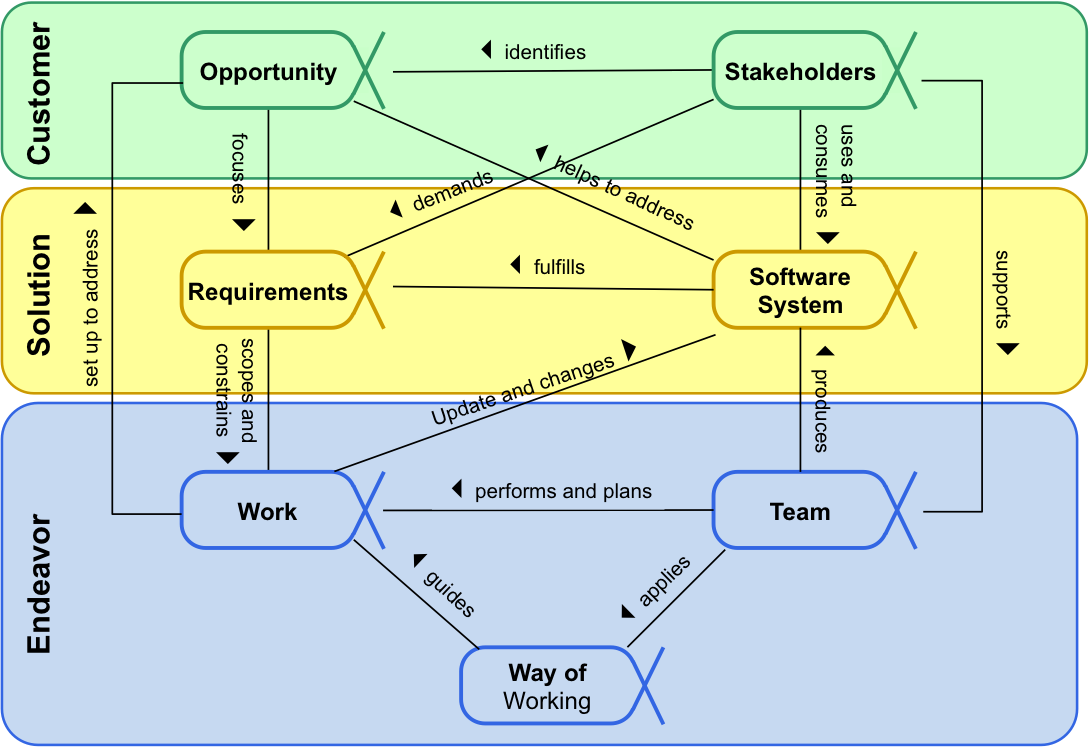
\includegraphics[width=0.8\textwidth]{img/prog}		
			\caption{Elementi di un progetto.}
		\end{figure} 
		
		
		\begin{figure}[H]
			\centering
			\subfloat[\underline{\hyperref[opportunity]{Opportunity}}.]{{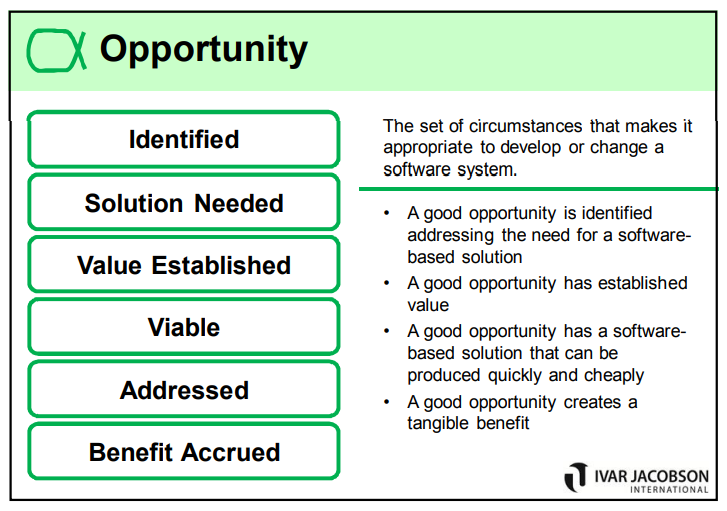
\includegraphics[width=0.46\textwidth]{img/cards/opp}	}}
			\qquad
			\subfloat[\underline{\hyperref[stakeholder]{Stakeholders}}.]{{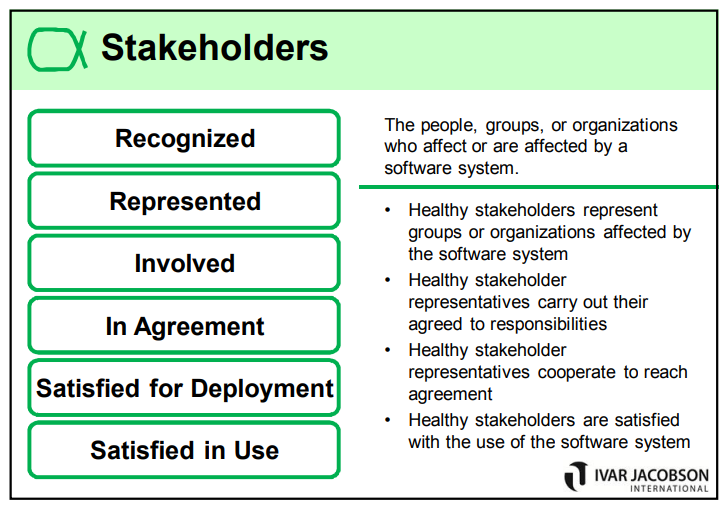
\includegraphics[width=0.46\textwidth]{img/cards/stake} }}
		\end{figure}
		
		\begin{figure}[H]
			\centering
			\subfloat[\underline{\hyperref[requirements]{Requirements}}.]{{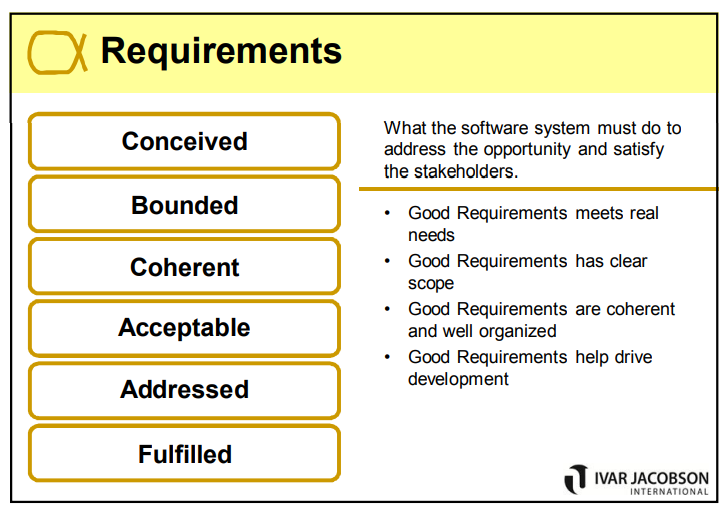
\includegraphics[width=0.46\textwidth]{img/cards/req}	}}		
			\qquad
			\subfloat[\underline{\hyperref[sistemasoftware]{Software System}}.]{{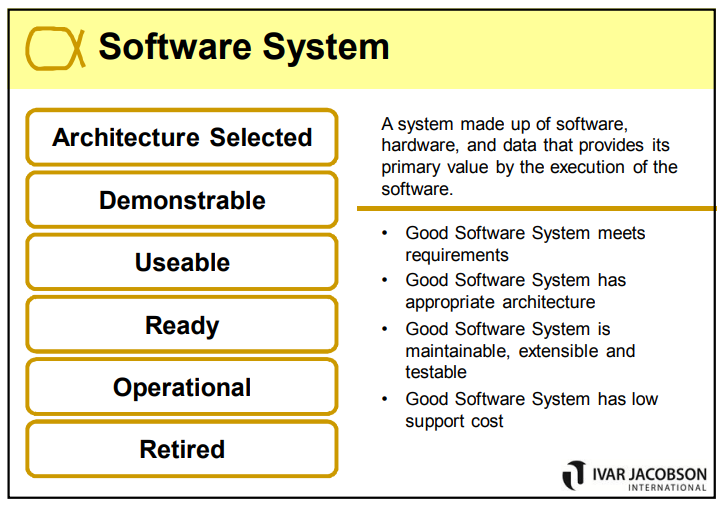
\includegraphics[width=0.46\textwidth]{img/cards/soft}	}}
		\end{figure} 
	
		\begin{figure}[H]
			\centering
			\subfloat[\underline{\hyperref[work]{Work}}.]{{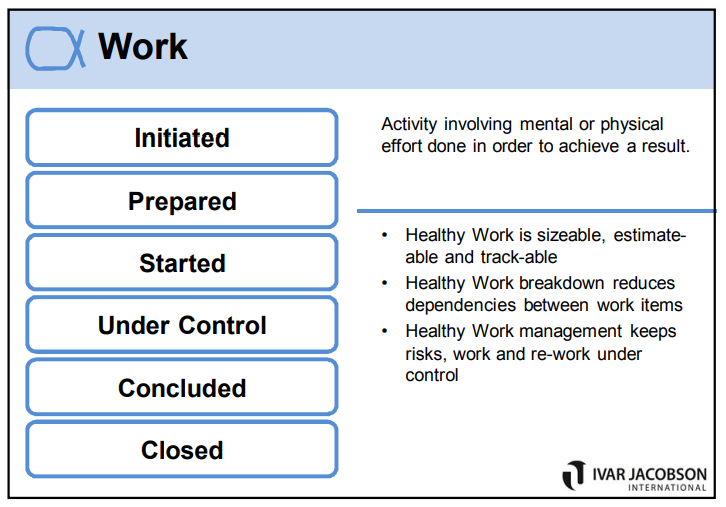
\includegraphics[width=0.46\textwidth]{img/cards/work}	}}		
			\qquad
			\subfloat[\underline{\hyperref[team]{Team}}.]{{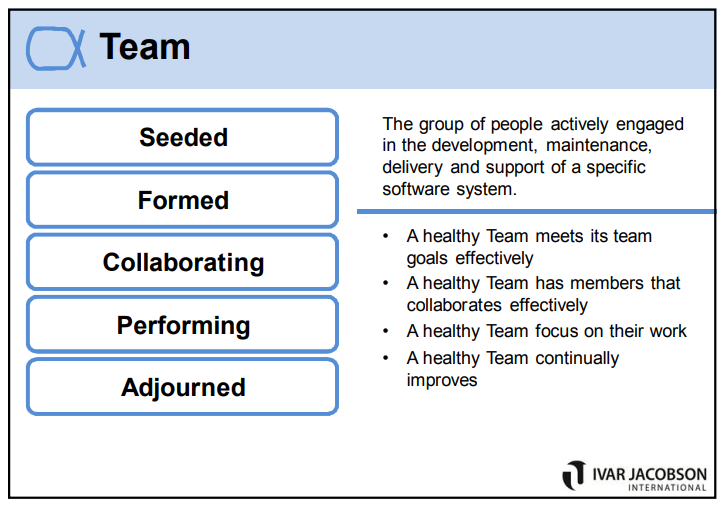
\includegraphics[width=0.46\textwidth]{img/cards/team}	}}
		\end{figure} 
	
		\begin{figure}[H]
			\centering
			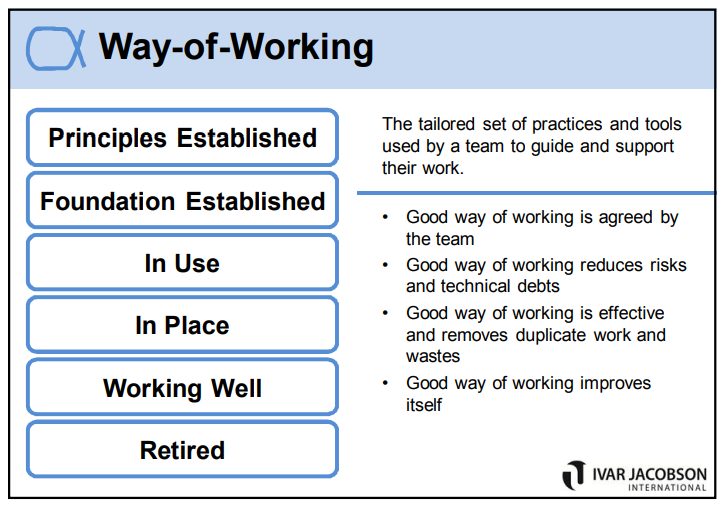
\includegraphics[width=0.46\textwidth]{img/cards/way}		
			\caption{\underline{\hyperref[way]{Way of working}}.}
		\end{figure} 
			
		Molto importante all'interno di un progetto è la \underline{\hyperref[gestioneprogetto]{Gestione di progetto}}. Per il progetto didattico vedi \underline{\hyperref[3p]{3P}}.
			
	%	\subsection{PROJECT-FIRST JUST-IN-TIME-PRINCIPLES APPROACH} \index{Project-first approach} \label{approach}
	%	Sfide maggiori se superate danno skills maggiori e maggior soddisfazione (ma non deve essere troppo alto e dare ansia, ma neanche troppo basso e annoiare).
		
		\subsection{PROGRAMMATORE} \index{Programmatore} \label{programmatore}
		È uno dei \underline{\hyperref[ruoli]{ruoli}} in un progetto. Sono la categoria più popolosa. Partecipano alla realizzazione e manutenzione del prodotto e hanno competenze tecniche, visione e responsabilità circoscritte.
		
		
		\subsection{PROGRAMMI VERIFICABILI}	\index{Programmi verificabili}	\label{programmiverificabili} %13 dicembre - verifica e validazione: analisi statica
		Serve dotarsi di uno standard di codifica coerente con le esigenze di \underline{\hyperref[verificare]{verifica}}. Per questo, per scrivere programmi verificabili, serve regolamentare l’uso del linguaggio di programmazione tramite principi da riflettere nelle Norme di Progetto:
		\begin{itemize}
			\item per assicurare \underline{\hyperref[comportamentopredicibile]{comportamento predicibile}};
			\item per usare \underline{\hyperref[criteriprog]{criteri di programmazione}} ben fondati;
			\item per \underline{\hyperref[pragmatico]{ragioni pragmatiche}};
		\end{itemize}
		Prima tecnica per essere sicuri: \underline{\hyperref[tracciamento]{tracciamento}}. \\
		Obblighi di analisi statica del codice: %slide 15/30
		\begin{itemize}
			\item \textbf{Analisi del flusso di controllo}: il modo in cui avanza il programma .%tramite il Program Counter?
			Alcune istruzioni cambiano il flusso (ad es: go to, cicli, ecc). Usare la ricorsione con grande parsimonia;
			\item\textbf{Analisi di flusso dei dati}: vedere l'ordine delle variabili. Si accerta che il programma non acceda a variabili prive di valore. Questa analisi è resa facile tramite incapsulazione. Non si fa eseguendo, ma prima. 
			\item \textbf{Analisi dei flusso d'informazione}: è il modo in cui valorizzo il dato. Determina la relazione tra ingressi e uscite di un'unità di codice. Bisogna capire se il valore informativo del dato è perso o meno.
			\item \textbf{Esecuzione simbolica}: dopo analisi di flusso di dati e d'informazione, so ora calcolare quale funzione dell'input produce l'output. L'uscita che vedo è la conseguenza di un flusso.
			\item \textbf{Verifica formale del codice}: usare le pre-condizioni e le post-condizioni e gli invarianti. Importante per vedere se il programma è corretto \textit{\underline{\hyperref[byconstruction]{by construction}}}; provare quindi la correttezza del codice sorgente rispetto alla specifica algebrica dei requisiti;
			\item \textbf{Analisi di limite}: limiti importanti sono overflow e underflow; rispetto dei limiti (fare \textit{range checking});
			\item \textbf{Analisi d'uso di stack}: Prima ragione di crescita: quando annido chiamate lo stack cresce. Lo stack è deciso all'elaborazione (quella è la massima estensione). Seconda ragione di crescita: i parametri che ci metto. Quando lo stack cresce oltre il suo confine cammina sull'heap, fare quindi attenzione che non tracimi [vedere le variabili del main dove stanno, se heap o stack];
			\item \textbf{Analisi temporale}: studiare le dipendenze temporali (latenza, tempestività) tra le uscite del programma e i suoi ingressi per verificare che il valore giusto sia prodotto al momento giusto;
			\item \textbf{Analisi d'interferenza}: mostrare l’assenza di effetti di interferenza tra parti isolate del sistema. Veicoli tipici di interferenza: memoria condivisa e I/O;
			\item \textbf{Analisi di codice oggetto}: assicurare che il codice oggetto da eseguire sia una traduzione corretta del codice e che non sia stata introdotta nessuna omissione dal compilatore;
		\end{itemize}
		
		
		\subsection{PROOF OF CONCEPT}	\index{Proof of Concept} \label{poc}
		Poc: risposta alle domande sulla fattibilità  della tecnologia selezionata. Prima di tutto capisco le domande e poi elaboro le risposte. Dimostro poi che il lavoro si può fare (rappresenta una \underline{\hyperref[baseline]{baseline}})e lo rendo accessibile al committente.
			
		\subsection{PROTOTIPO} \index{Prototipo} \label{prototipo}
		Dà l'idea di ció che sarà il \underline{\hyperref[prodotto]{prodotto}}. Serve per provare e scegliere possibili soluzioni. Può essere usato in modo \underline{\hyperref[incremento]{incrementale}} come la baseline, o "usa e getta" quindi \underline{\hyperref[iterazione]{iterativo}}).
		
		\subsection{PROVA}	\index{Prova}	\label{prova} %slide 13
		Una prove eseguibile è una procedura applicata a una \underline{\hyperref[testsuite]{batteria di prove}}.
	
	

	\newpage
	\flushright{\hyperref[index]{\color{black!65}{Ritorna all'indice}}}\flushleft
	\section{Q} \label{sec:Q}
	
		\subsection{QUALIFICA} \index{Qualifica} \label{qualifica}
		Verifica + validazione.  
	
		\subsection{QUALITÀ} \index{Qualità} \label{qualita} %V.I
		L’insieme delle proprietà e delle caratteristiche di un prodotto che conferiscono ad esso la capacità di soddisfare esigenze espresse o implicite del cliente. Serve per emancipare. Si vede chi fa (sulla base di qualche riferimento), chi usa (almeno il minimo obbligatorio) e chi valuta (etichettano).
		La qualità è di prodotto e di processo.
		Per quel che riguarda la \textit{qualità di prodotto} esistono:
		\begin{itemize}
			\item \textit{Sistema di Qualità}: è la struttura organizzativa e le risorse messe in atto per perseguire la qualità, in cui c'è la supervisione di miglioramento continuo;
			\item \underline{\hyperref[pianoqualita]{Piano della Qualità}};
			\item \underline{\hyperref[controlloqualita]{Controllo di qualità}};				
		\end{itemize}
		Il modello di sviluppo muove il ciclo. Vogliamo vedere quanto abbiamo consumato per raggiungere quella quantità. \\
		La qualità è un poliedro: ha tante facce ed è in stretta correlazione a \underline{\hyperref[efficacia]{efficacia}} e \underline{\hyperref[valutazione]{valutazione}} . \\
		Riguardo alla \textit{qualità di processo} bisogna definire il \underline{\hyperref[processo]{processo}} per controllarlo e migliorarne efficacia, efficienza ed esperienza. Usare inoltre buone metriche e strumenti di valutazione. Ci riferiamo qui ora allo \underline{\hyperref[standard]{standard}} ISO 9000. Esiste inoltre un \underline{\hyperref[manualequalita]{Manuale della qualità}} e degli strumenti di valutazione tra cui:
		\begin{itemize}
			\item \textbf{SPY}: \textit{SW Process Assessment and Improvement}, dà una valutazione oggettiva dei processi di una organizzazione per darne un giudizio di maturità e individuare azioni migliorative;
			\item \textbf{\underline{\hyperref[cmmi]{CMMI}}};
			\item \textbf{\underline{\hyperref[15504]{ISO 15504}}};
		\end{itemize}
	
	

	\newpage
	\flushright{\hyperref[index]{\color{black!65}{Ritorna all'indice}}}\flushleft
	\section{R} \label{sec:R}
	
		\subsection{READY}	\index{Ready}	\label{ready}
		Vuol dire che nessuna parte manca e la documentazione è pronta. Gli stakeholder hanno accettato il prodotto e vogliono che diventi operativo.
	
		\subsection{REALIZZAZIONE} \index{Realizzazione}	\label{realizzazione}
		Attua ciò che è stato progettato durante la \underline{\hyperref[progettazione]{Progettazione Software}}: avviene quindi la stesura del codice SENZA INVENTARE. Infine avviene l'attività di collaudo che è il nostro passo di uscita sapendo l'esito che avrà.
		
		\subsection{REQUIREMENTS} \index{Requirements} \label{requirements}
		Idea di soluzione per soddisfare il bisogno (quindi astratta).
		È la descrizione documentata di una \textbf{capacità}
		\begin{itemize}
			\item necessaria a un utente per raggiungere un obiettivo (vista dal lato del cliente);
			\item che un sistema deve possedere per adempiere a un obbligo (vista dal lato dello sviluppatore). 
		\end{itemize}
	
	    I requisiti devono essere tutti identificabili e verificabili. Vengono classificati, per facilitare la comprensione, la \underline{\hyperref[manutenzione]{manutenzione}} e il \underline{\hyperref[tracciamento]{tracciamento}}, in base ad
	    	\begin{itemize}
	    		\item \textbf{attributi di prodotto}: rispondono a \textit{Cosa devo fare?} (requisiti funzionali, prestazionali e di qualità);
	    		\item \textbf{attributi di processo}: rispondono a \textit{Come devo farlo?} (requisiti di vincolo);
	    	\end{itemize}
	    
		Ogni tipo di requisito può essere diretto o indiretto, implicito o esplicito ma ognuno deve essere \underline{\hyperref[verificare]{verificabile}} tramite:
		\begin{itemize}
			\item \textbf{per requisiti funzionali}: test, dimostrazione frontale, revisione;
			\item \textbf{per requisiti prestazionali}: misurazione;
			\item \textbf{per requisiti qualitativi}: tecniche ad hoc;
			\item \textbf{per requisiti dichiarativi(vincoli)}: revisione.
		\end{itemize}
	
		In base all'utilità strategica possono inoltre essere classificati in:
		\begin{itemize}
			\item \textbf{obbligatori}: irrinunciabili secondo gli \underline{\hyperref[stakeholder]{stakeholder}};
			\item \textbf{desiderabili}: non strettamente necessari ma danno valore aggiunto; 
			\item \textbf{opzionali}: relativamente utili.
		\end{itemize}
		Questo perché devo capire quali requisiti sono irrinunciabili. I requisiti sono quindi elastici e dipendono da me, da quanto sono veloce, ecc.
			
		\underline{\hyperref[qualita]{Qualità}} che ci devono essere secondo \underline{\hyperref[ieee830]{IEEE 830}}:
		\begin{itemize} %slide 25/32
			\item \textbf{non ambiguo} ovvero il requisito deve essere scritto in maniera concisa per non creare confusione (ma attenzione perché non c'é una metrica);
			\item \textbf{corretto};
			\item \textbf{completo} c'è tutto ciò che ci deve essere;
			\item \textbf{verificabile};
			\item \textbf{consistente} perché non possono essere contraddittori;
			\item \textbf{modificabile} con la \underline{\hyperref[gestionecambiamenti]{Gestione dei cambiamenti}}, ma l'indice che ogni requisito ha non lo do io (altrimenti se modifico qualcosa devo riordinare tutto) e deve essere significativo;
			\item \textbf{tracciabile};
			\item \textbf{ordinato per prevalenza};		
		\end{itemize}	
	
		Durante l'\underline{\hyperref[analisideirequisiti]{Analisi dei requisiti}} avviene inoltre la \underline{\hyperref[verificare]{verifica}} dei requisiti:
			\begin{itemize}
				\item Viene eseguita su un documento organizzato tramite \underline{\hyperref[walkthrough]{walkthrough}} o \underline{\hyperref[inspection]{ispezione}} (lettura mirata);
				\item Si ricerca chiarezza espressiva, che non è il linguaggio naturale;
				\item Si ricerca chiarezza strutturale, ovvero si controlla la separazione tra requisiti funzionali e non-funzionali e che la \underline{\hyperref[classificazione]{classificazione dei requisiti}} sia precisa, uniforme e accurata;
				\item Si ricerca atomicità e aggregazione, quindi i requisiti elementari e le correlazioni tra di essi chiare ed esplicite;
			\end{itemize}
		
		Anche la \underline{\hyperref[gestionerequisiti]{Gestione dei requisiti}}.
		
		\subsection{RESPONSABILE} \index{Responsabile} \label{responsabile}
		È uno dei \underline{\hyperref[ruoli]{ruoli}} in un progetto. Partecipa al \underline{\hyperref[progetto]{progetto}} per tutta la sua durata rappresentando il progetto presso il fornitore e il committente. Accentra le responsabilità di scelta e approvazione, quindi deve avere conoscenze e capacità tecniche per valutare (rischi e scelte varie). Ha molte responsabilità, nello specifico su: \underline{\hyperref[pianificazione]{Pianificazione}}, gestione delle risorse umane, controllo, coordinamento e relazioni con l'esterno.
		
		\subsection{REVISIONE DEI REQUISITI} \index{Revisione dei Requisiti} \label{RR} 
		1. \\
		Ha la funzione di concordare con il cliente una visione condivisa del prodotto atteso.
		Prevede:
		\begin{itemize}
			\item \underline{\hyperref[analisideirequisiti]{Analisi dei Requisiti}};
			\item \underline{\hyperref[piano]{Piano}} di Progetto;
			\item Piano di Qualifica;
			\item \underline{\hyperref[norme]{Norme di Progetto}};
			\item \underline{\hyperref[studiofattibilita]{Studio di Fattibilità}};
		\end{itemize}
		Fa l'\underline{\hyperref[audit]{Audit Process}}.
		
		\subsection{REVISIONE DI ACCETTAZIONE} \index{Revisione di Accettazione} \label{RA} 
		4. \\
		Ha la funzione di collaudare il sistema per accettazione da parte del committente e accertarsi del soddisfacimento di tutti i requisiti utente fissati nella RR.
		Prevede:
		\begin{itemize}
			\item \underline{\hyperref[productbaseline]{Product Baseline}};
			\item \underline{\hyperref[piano]{Piano}} di Qualifica (quarta versione);
			\item \underline{\hyperref[piano]{Piano}} di Progetto (quarta versione) con \underline{\hyperref[consuntivo]{consuntivo}} finale;
			\item \underline{\hyperref[manuali]{Manuale}} Utente e Manuale Sviluppatore (entrambe seconda versione);
		\end{itemize}
		Fa l'\underline{\hyperref[audit]{Audit Process}}.
		
		\subsection{REVISIONE DI PROGETTAZIONE}	\index{Revisione di Progettazione} \label{RP}
		2. \\
		Ha la funzione di accertare la realizzabilità.
		Prevede:
		\begin{itemize}
			\item \underline{\hyperref[technologybaseline]{Technology Baseline}};
			\item \underline{\hyperref[piano]{Piano}} di Qualifica (seconda versione);
			\item \underline{\hyperref[piano]{Piano}} di Progetto (seconda versione);
			\item \underline{\hyperref[norme]{Norme di Progetto}} (seconda versione);
		\end{itemize}
		Fa l'\underline{\hyperref[joint]{Joint Review Process}}.
		
		\subsection{REVISIONE DI QUALIFICA} \index{Revisione di Qualifica} \label{RQ} 
		3. \\
		Ha la funzione di approvare l’esito finale delle verifiche e attivare la validazione.
		Prevede:
		\begin{itemize}
			\item \underline{\hyperref[productbaseline]{Product Baseline}};
			\item \underline{\hyperref[piano]{Piano}} di Qualifica (terza versione);
			\item \underline{\hyperref[piano]{Piano}} di Progetto (terza versione);
			\item \underline{\hyperref[manuali]{Manuale}} Utente e Manuale Sviluppatore;
			\item eventuale \underline{\hyperref[norme]{Norme di Progetto}} (terza versione);
		\end{itemize}
		Fa l'\underline{\hyperref[joint]{Joint Review Process}}.
		
		\subsection{RIUSO} \index{Riuso} \label{riuso} 
		Il riuso può qui essere:
			\begin{itemize}
				\item \textbf{occasionale} perchè "copia e incolla" opportunistico, che ha quindi un basso costo ma scarso impatto;
				\item \textbf{sistematico} perchè è un "copia e incolla" intelligente, che ha un maggior costo ma maggior impatto;
			\end{itemize}
		Nel breve periodo il riuso diventa più un costo.
		
		
		\subsection{RUOLI} \index{Ruoli} \label{ruoli} 
		Il ruolo è una persona che si occupa di una funzione aziendale assegnata in un progetto. Tra queste funzioni aziendali troviamo: \textit{Sviluppo} quindi avere responsabilità tecnica e realizzativa, \textit{Direzione} quindi avere responsabilità decisionale, \textit{Amministrazione} ovvero gestione del supporto ai processi e \textit{\underline{\hyperref[qualita]{Qualità}}} quindi gestione della ricerca di economicità.
		A seguire, l'elenco dei ruoli all'interno della \underline{\hyperref[gestioneprogetto]{gestione del progetto}} (ricordiamo che non vogliamo sovrapposizioni):
		\begin{itemize}
		\item \textbf{\underline{\hyperref[analista]{Analista}}}: fa l'analisi dei requisiti. Capisce ciò di cui c'è bisogno per cui è importante che si metta nei panni dell'utente.
		\item \textbf{\underline{\hyperref[progettista]{Progettista}}}: pensa ad una possibile soluzione con qualità desiderabili (ATTENZIONE: non implementa).
		\item \textbf{\underline{\hyperref[programmatore]{Programmatore}}}: concretizza la soluzione che il progettista ha pensato (ATTENZIONE: non inventa).
		\item \textbf{\underline{\hyperref[verificatore]{Verificatore}}}: dice se il lavoro del programmatore è conforme alle attese. Deve poi relazionarsi ed essere di supporto.
		\item \textbf{\underline{\hyperref[responsabile]{Responsabile}}}: "onere e onore" in particolare ha tanti oneri. Coordina il team e garantisce che non ci siano intoppi o rallentamenti.
		\item \textbf{\underline{\hyperref[amministratore]{Amministratore}}}: garantisce che funzioni bene il nostro sistema informatico (che sia scalabile, ecc).
		\end{itemize}		
	
	

	\newpage
	\section{S} \label{sec:S}

		\subsection{SCALABILITÀ} \index{Scalabilità} \label{scalabitlita}
		È la caratteristica di un sistema software o hardware facilmente modificabile nel caso di variazioni notevoli della mole o della tipologia dei dati trattati. \\
		Garantisce prestazioni.


		\subsection{SEMAT} \index{SEMAT} \label{semat}
		\textit{Software Engineering Method and Theory} fornisce teorie, principi provati e \underline{\hyperref[best]{best practices}} per l'Ingegneria del Software.


		\subsection{SISTEMA DI QUALITÀ} \index{Sistema di qualità} \label{sistemadiqualita}
		Riferimenti \textbf{oggettivi} che ci dicono come stiamo lavorando.


		\subsection{SLACK} \index{Slack} \label{slack}
		Significato letterale:``lasco''. Con questo si intende il margine che posso consumare (per esempio, nel caso di un ritardo di attività che devo finire di completare).


		\subsection{SOFTWARE DETERMINISTICO} \index{Software deterministico} \label{softwaredeterministico}
		In ogni stato del prodotto SW in cui mi trovo, so che posso avere solo ``un'unica e sola uscita''. Devo sempre sapere lo stato in cui sono, quindi avere ben chiaro quello precedente e quello seguente.


		\subsection{SOFTWARE ENGINEERING} \index{Software Engineering} \label{swe}
		 L'\underline{\hyperref[engineering]{Ingegneria}} del Software è una disciplina volta a realizzare  \underline{\hyperref[prodotto]{prodotti software}} talmente impegnativi da richiedere lo svolgimento di attività collaborative. Agisce garantendo \underline{\hyperref[efficacia]{efficacia}} ed \underline{\hyperref[efficienza]{efficienza}} durante tutto il \underline{\hyperref[ciclo]{ciclo di vita}} del prodotto. \\
		 È importante sottolineare che l'Ingegneria del Software non ha a che vedere solo con l'informatica, ma anche con alcune aree della matematica discreta, ricerca, statistica, psicologia ed economia. L'Ingegneria del Software inoltre adotta un determinato \underline{\hyperref[approccio]{approccio}}.


		\subsection{SOFTWARE SYSTEM} \index{Sistema software} \label{sistemasoftware}
		Soluzione realizzabile (concretizza \underline{\hyperref[requirements]{requirements}}).


		\subsection{SOLUTION} \index{Solution} \label{solution}
		Secondo elemento di un \underline{\hyperref[progetto]{progetto}} secondo \underline{\hyperref[semat]{SEMAT}}. Esso comprende \underline{\hyperref[requirements]{requirements}} e
		 \underline{\hyperref[sistemasoftware]{software system}}.

		\subsection{STAKEHOLDER} \index{Stakeholder} \label{stakeholder}
		Traduzione di \textit{portatori di interesse}, sono le persone influenti per il prodotto: dicono se una certa \underline{\hyperref[opportunity]{opportunità}} è buona.
		Possono essere chi usa il prodotto (cliente), chi compra il prodotto (committente), chi sostiene i costi di realizzazione (fornitore), chi verifica l'attuazione di processi (eventuali regolatori). \\
		È uno degli elementi di un progetto (vedi \underline{\hyperref[customerimage]{immagine}}).

		\subsection{STANDARD DI PROCESSO} \index{Standard di processo} \label{standard}
		Nascono per iniziativa del committente al fine di facilitare controllo, collaudo e accettazione.
		Esistono standard come:
		\begin{itemize}
			\item \textbf{Modello di azione}: definiscono procedure o processi
			\item \textbf{Modello di valutazione}: sono modelli più generali e identificano la \underline{\hyperref[best]{best practice}}
		\end{itemize}


			\subsubsection{STANDARD IEEE 830-1998}	\index{Standard IEEE 830-1998} \label{ieee830}
			Questo standard delinea la struttura che deve avere il documento \underline{\hyperref[analisideirequisiti]{Analisi dei Requisiti}} e le \underline{\hyperref[qualita]{qualità}} che devono possedere i requisiti.
			\textit{Recommended Practice for Software Requirements Specifications} dice che la specifica deve essere:
				\begin{itemize}
					\item Priva di ambiguità
					\item Corretta
					\item Completa
					\item Verificabile
					\item Consistente
					\item Modificabile
					\item Tracciabile
					\item Ordinata per rilevanza
				\end{itemize}
			Per la restante documentazione relativa alla struttura dell'AdR, vedere il \href{https://www.cs.purdue.edu/homes/apm/courses/BITSC461-fall03_SoftwareEngineering/miller-guidelines/IEEE830-1998.html}{link qui}.


			\subsubsection{STANDARD ISO 12207}	\index{Standard ISO 12207}	\label{12207}
			È un \textit{modello di azione} ed il modello più noto. Contiene tutti i processi significativi ad alto livello:
			\begin{itemize}
				\item Identifica i processi di ciclo di vita del \underline{\hyperref[prodotto]{software}}
				\item Ha struttura modulare
				\item Specifica le responsabilità sui processi
				\item Specifica i prodotti dei processi
			\end{itemize}

			\begin{figure}[H]
				\centering
				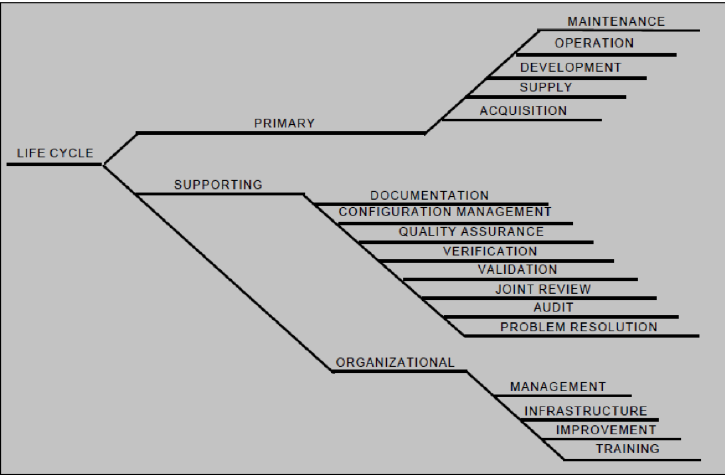
\includegraphics[width=0.78\textwidth]{img/iso}
				\caption{Primary, supporting and organisational life-cycle processes.}
			\end{figure}

			Almeno un \textit{processo primario} deve sempre esistere:
				\begin{itemize}
					\item \textbf{Acquisizione}: gestione dei sotto-fornitori
					\item \textbf{Fornitura}: gestione dei rapporti con il cliente
					\item \textbf{Sviluppo}: non è sempre detto che abbia rapporti con il cliente
					\item \textbf{Gestione operativa/utilizzo}: installazione ed erogazione dei prodotti
					\item \textbf{\underline{\hyperref[manutenzione]{Manutenzione}}}
				\end{itemize}

			\textit{Processi di supporto}:
				\begin{itemize}
					\item \textbf{Documentazione}
					\item \textbf{Accertamento della \underline{\hyperref[qualita]{qualità}}}
					\item \textbf{Gestione delle \underline{\hyperref[versione]{versioni}} e delle \underline{\hyperref[configurazione]{configurazioni}}}
					\item \textbf{\underline{\hyperref[verificare]{Verifica}}}
					\item \textbf{\underline{\hyperref[validare]{Validazione}}}
					\item \textbf{Revisioni congiunte con il cliente}
					\item \textbf{Verifiche ispettive interne}
					\item \textbf{Risoluzione dei problemi}: con gestione dei problemi
				\end{itemize}

			Trasversali rispetto ai singoli progetti sono invece i \textit{processi organizzativi}:
				\begin{itemize}
					\item \textbf{Gestione dei processi}
					\item \textbf{Gestione delle infrastrutture}
					\item \textbf{Miglioramento del processo}
					\item \textbf{Formazione del personale}
				\end{itemize}

			%La soluzione dei problemi... problem solution.	%slide 10/22


			\subsubsection{STANDARD ISO 14598}	\index{Standard ISO 14598}	\label{14596}
			ISO/IEC 14598:1999 fornisce il \textit{modello di valutazione} che non cambia nel tempo e col contesto. La metrica che adotta è un modo
			%per mettere in scala i numeri,
			per dare un significato condiviso e non ambiguo a delle caratteristiche.


			\subsubsection{STANDARD ISO 15504}	\index{Standard ISO 15504}	\label{15504}
			\textit{Software Process Improvement Capability dEtermination} \\
			Standard di \underline{\hyperref[qualita]{qualità}} nato per armonizzare 12207 e 9001. È un \textit{modello di valutazione} e si occupa di:
			\begin{itemize}
				\item \textbf{Identificazione degli stakeholder}: destinatari dei risultati, responsabili dei processi valutati
				\item \textbf{Scelta tra valutazione e miglioramento}: risultato a uso esterno o interno, approccio formale (\underline{\hyperref[audit]{\textit{audit}}}) o meno (\textit{self-assessment})
				\item \textbf{Definizione della portata}: processi inclusi nella valutazione e indicatori di valutazione
			\end{itemize}


			\subsubsection{STANDARD ISO 15939}	\index{Standard ISO 15939}	%slide 10 - Misurazione del software
			(Sappiamo solo che esiste ma non è da usare perchè è costoso) \\
			Misura e ha forma di ciclo, quindi non ha fine.
			%Si passa sempre per il punto di Management processes.
			Il mio cruscotto cambia in base al contesto, non è scelto a priori e basta, se no diventa vecchio (esempio: quando faccio codice guardo la qualità per il codice, quando faccio requisiti ho un altro cruscotto).


			\subsubsection{STANDARD ISO 25000}	\index{Standard ISO 25000}	\label{2500}
			ISO/IEC 25000:2014 è un insieme dello standard 9126 e 14598.
			Si riferisce al software, \textit{SQuaRE}: \textit{Software product Quality Requirements and Evaluation}.


			\subsubsection{STANDARD ISO 9000}	\index{Standard ISO 9000}	\label{9000}
			La famiglia delle norme ISO 9000 tratta i fondamenti dei modelli di qualità, neutri rispetto al dominio di applicazione.

			\begin{figure}[H]
				\centering
				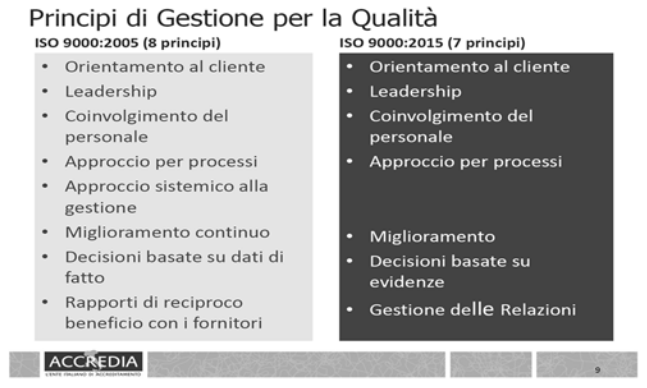
\includegraphics[width=0.65\textwidth]{img/9000}
				\caption{I principi ISO 9000.}
			\end{figure}


			\subsubsection{STANDARD ISO 9001}	\index{Standard ISO 9001}	\label{9001}
			Applica lo standard 9000 ai sistemi produttivi. È la certificazione per la valutazione dei fornitori di prodotti o servizi. \\
			Per il miglioramento dei risultati è stato in seguito creato il 9004.


			\subsubsection{STANDARD ISO 9126}	\index{Standard ISO 9126}	\label{9126} % slide 13/22 Set Qualità
			Standard per la qualità del prodotto.
			Fatto di due parti:
				\begin{itemize}
					\item Come si definiscono le caratteristiche rilevanti
					\item Come si misurano (con quali \underline{\hyperref[metrica]{metriche}}) per poterle valutare
				\end{itemize}
			Tre diverse visioni tutte da considerare:
				\begin{itemize}
					\item \textbf{Visione esterna}: ciò che si osserva del prodotto relativo all'esecuzione
					\item \textbf{Visione interna}: come è fatto rispetto a cosa fa
					\item \textbf{Visione in uso}: come vedo il prodotto quando devo usarlo
				\end{itemize}

			\begin{figure}[H]
				\centering
				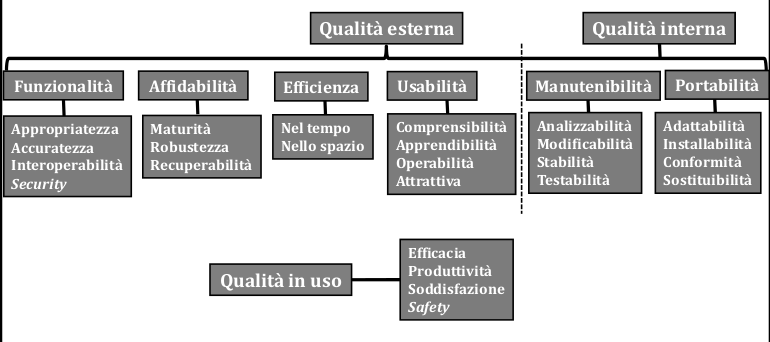
\includegraphics[width=0.78\textwidth]{img/9126}
				\caption{Le diverse visioni delle qualità di ISO 9126:2001.}
			\end{figure}


		\subsection{STATEMENT COVERAGE}	\label{statementcoverage}	\index{Statement Coverage}
		Strumento che si ricorda quali \textit{statement} il test ha attraversato. Si ha quindi copertura al 100\% quando i test effettuati sull'unità sono sufficienti a eseguire almeno una volta tutti i comandi dell'unità con esito corretto. \\
		(Un esempio di differenza con \underline{\hyperref[branchcoverage]{branch coverage}} su \href{https://stackoverflow.com/questions/14519416/a-difference-between-statement-and-decision-coverage}{StackOverflow}).


		\subsection{STATO} \index{Stato} \label{stato}
		%[Da Automi] \\
		È il valore assunto da variabili di stato, conseguente ad azioni precedenti su di esse. Viene deciso dal \textit{Software Engineer}.

		\subsection{STUB}	\index{Stub}	\label{stub}
		Sono dei sostituti (come i \underline{\hyperref[mock]{mock}}), ovvero rappresentano ciò che è chiamato dal test, ma che ancora non c'è (per esempio evita ClassNotFound).

		\subsection{STUDIO DI FATTIBILITÀ} \index{Studio di fattibilità} \label{studiofattibilita}
		Non è un documento pubblico, ma deve rimanere agli atti come un ragionamento ben fondato.
		È quindi un prodotto interno e definisce il rapporto tra le parti. \\
		Si capisce qui cosa si è capaci di fare, perché innanzitutto si valutano rischi, costi e benefici nell'ottica del cliente e del fornitore.
		Si valuta se procedere, con l’obiettivo di restare entro un costo massimo prefissato e con le conoscenze immediatamente disponibili o un piano di formazione.
		Si studiano:
		\begin{itemize}
			\item Gli strumenti e le tecnologie per la realizzazione
			\item Le soluzioni algoritmiche e architetturali
			\item Le piattaforme idonee all'esecuzione
			\item Il costo di produzione rispetto alla redditività
		\end{itemize}
		Inoltre le attività che vengono fatte sono:
		\begin{itemize}
			\item Individuazione dei rischi
			\item Valutazione delle scadenze temporali (con conseguente studio delle risorse disponibili rispetto a quelle necessarie)
			\item Valutazione delle possibili strategie alternative
		\end{itemize}

	\newpage
	\section{T} \label{sec:T}

		\subsection{TASK} \index{Task} \label{task}
		È l'equivalente inglese di \textit{attività}: complesso di azioni dirette alla realizzazione di un obiettivo. \\
		È diverso da compito: parte di lavoro che si assegna ad altri o che qualcuno prefigge a se stesso di fare.

		\subsection{TECHNOLOGY BASELINE} \index{Technology Baseline} \label{technologybaseline}
		Dimostrare, al committente e a noi stessi, di disporre delle tecnologie, librerie e framework necessari per lo sviluppo del prodotto, portando una baseline.
		Ne dimostriamo l'adeguatezza tramite \underline{\hyperref[poc]{Proof of Concept}} ed è soggetta a verifica Agile. \\
		Fa parte del periodo di \underline{\hyperref[RP]{RP}}.

		\subsection{TEMPO/PERSONA} \index{Tempo/persona} \label{tempopersona}
		Quanto tempo produttivo sta usando quella persona (o profilo). La sommatoria mi dà il costo complessivo.

		\subsection{TEST} \index{Test}	\label{test}	%7 dicembre - Verifica e validazione
		Prima di mettere insieme tutti i vari programmi in un prodotto SW, bisogna accertarsi che ogni piccola parte funzioni tramite test. %slide 5/22 set verifica e validazione
		Per questo conviene adottare la \textit{Continuous Integration} che è una metodologia intelligente. Essa mi fa scegliere prima i vari test che mi andranno a testare una piccola parte di programma, poi quelli a cui al momento ne manca ancora un'altra (esempio: l'interfaccia senza database). \\
		I principali tipi di test sono:
		\begin{itemize}
			\item \underline{\hyperref[testunita]{Test di unità}}
			\item \underline{\hyperref[testintegrazione]{Test d'integrazione}}
			\item \underline{\hyperref[testsistema]{Test di sistema}}
			\item \underline{\hyperref[testregressione]{Test di regressione}}
			\item Test di accettazione (\underline{\hyperref[collaudo]{collaudo}})
		\end{itemize}
		E devono essere:
		\begin{itemize}
			\item \textbf{Ripetibili}: per questo si specifica ambiente di esecuzione, attese e procedure
			\item \textbf{Automatizzati}: per questo si usano strumenti come \textit{\underline{\hyperref[driver]{driver}}}, \textit{\underline{\hyperref[stub]{stub}}} e \textit{\underline{\hyperref[logger]{logger}}} (sono \underline{\hyperref[mock]{mock}})
			\item \textbf{Oggettivi}: non personalizzati
		\end{itemize}
		Ma fare i test in modo esaustivo è impossibile. \\
		\textbf{N.B:} tutte le regole dei test vengono decise nella progettazione.

		\begin{figure}[H]
			\centering
			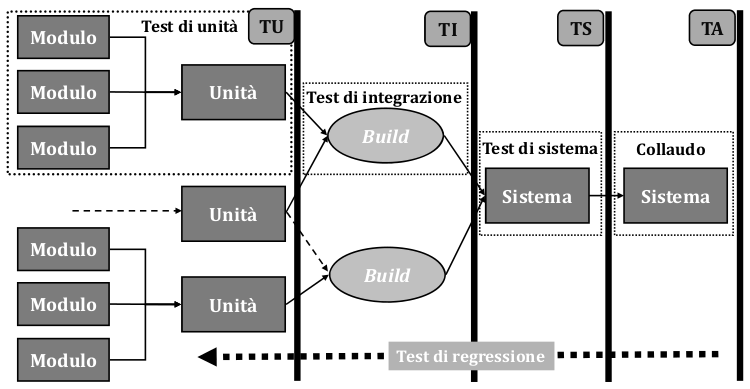
\includegraphics[width=0.9\textwidth]{img/test}
			\caption{Tipi di test (analisi dinamica).}
		\end{figure}
		%analisi dinamica % 20 dicembre
		I test comportano l'esecuzione dell'oggetto di verifica e devono dare misure di \underline{\hyperref[qualita]{qualità}}. Ogni test deve avere un obiettivo:
		\begin{itemize}
			\item Chiaro
			\item Utile
			\item Decidibile, perché c'è l'\underline{\hyperref[oracolo]{oracolo}}, ovvero deve produrre un esito verificato rispetto a un comportamento atteso
		\end{itemize}
		E il posto in cui inserisco queste cose è il \underline{\hyperref[pianoqualifica]{piano di qualifica}} (rispettando il \underline{\hyperref[V]{modello a V}}, ovvero prima definisco i test di validazione e sistema, poi quelli d'integrazione e infine i test di unità).

		Il verificatore controlla se ci sono problemi nei test. Se ci sono, essi sono dovuti a:
		\begin{enumerate}
			\item \underline{\hyperref[mistake]{Mistake}}
			\item \underline{\hyperref[fault]{Fault}}
			\item \underline{\hyperref[error]{Error}}
			\item \underline{\hyperref[failure]{Failure}}.
		\end{enumerate}
		Più obiettivi ha un test e peggio è (perché diventa difficile realizzarlo, farne il tracciamento, ecc).
		Più semplice è il SW da scrivere, più semplice sarà il test. \\
		La strategia richiede di trovare un bilanciamento tra la quantità minima e massima di casi di \underline{\hyperref[prova]{prova}} rispettando la legge del \underline{\hyperref[diminishingreturn]{rendimento decrescente}}.
		È importante perché i test costano e questo non è banale. \\
		Secondo Bertrand Meyer: \textit{``bisogna smantellare quello che ha in pancia un fault''}, ovvero bisogna sempre cercare di far fallire un test. \\ %..slide 13/34

		I test si specificano (\textit{Specifica}), poi vanno tradotti in (\textit{Codifica}) un eseguibile (da Codifica in poi voglio automatizzazione), collegati all'oggetto di test (\textit{Compilazione}), devo farli eseguire (\textit{Esecuzione}) e registrare l'esito (\textit{Analisi}). Infine l'output di un test si mette in un file chiamato file di log.

		\begin{figure}[H]
			\centering
			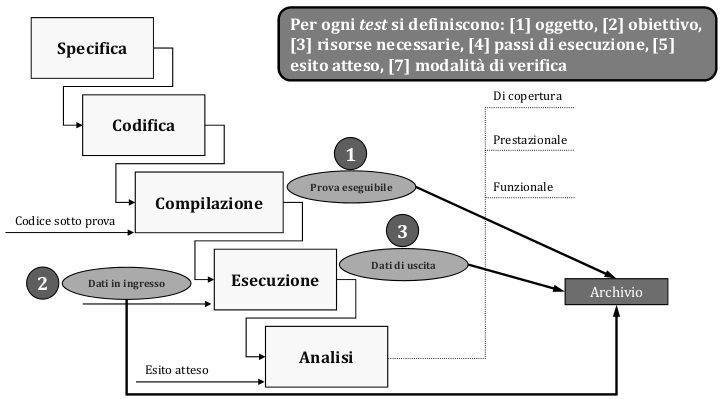
\includegraphics[width=0.8\textwidth]{img/prove}
			\caption{Attività di prova.}
		\end{figure}

		Si lavora per classi di equivalenza, in particolare 3:
		\begin{itemize}
			\item Valori non ammessi
			\item Valori barriera
			\item Valori ammessi entro barriere
		\end{itemize}
		Ogni insieme ha un rappresentate nei test.
		È facile ordinare gli interi qui dentro le classi di equivalenza, ma non altri valori come i numeri reali. \\
		Esistono inoltre 2 categorie di test principali:
		\begin{itemize}
			\item \textbf{Funzionale}: \textit{black-box} si occupa di vedere il tipo di uscita di quel test e credere che al suo interno vada tutto bene
			\item \textbf{Strutturale}: \textit{white-box} si occupa di cosa fa il test e non dell'effetto che produce, ricercando la massima copertura
		\end{itemize}
		Puntiamo ad avere massima copertura tramite i due \textit{coverage} (fattori di copertura): %slide 30/34
		\begin{itemize}
			\item \textbf{\underline{\hyperref[statementcoverage]{Statement Coverage}}}
			\item \textbf{\underline{\hyperref[branchcoverage]{Branch Coverage}}}
		\end{itemize}
		È difficile avere proprio il 100\%, quindi aver soddisfatto tutti i requisiti è tecnicamente impossibile, anche se è il nostro obiettivo.


		\subsection{TEST CASE}	\index{Test case}	\label{testcase}
		È una singola specifica di un singolo \underline{\hyperref[test]{test}}. \textit{Case} è un ``insieme di'' e, più specificatamente, un insieme di parametri:
		\begin{itemize}
			\item Ingresso
			\item Uscita
			\item Oggetto di prova
			\item Ambiente di sviluppo
		\end{itemize}


		\subsection{TEST DI INTEGRAZIONE}	\index{Test di integrazione} \label{testintegrazione}
		Verifica il residuo, che non possiamo accettare da una componente singola, mettendo insieme due unità con una \textit{build}.
		Sono idealmente quindi parti indipendenti messe insieme per collaborare, coese.
		L'integrazione, se c'è una buona architettura, è anche parallelizzabile. \\
		La \textit{logica} di integrazione funzionale:
		\begin{enumerate}
			\item Seleziona le funzionalità da integrare
			\item Identifica le componenti che svolgono quelle funzionalità
			\item Ordina le componenti per numero di dipendenze crescenti
			\item Esegue l'integrazione in quel determinato ordine.
		\end{enumerate}
		Più test di questo tipo faccio, più piccola è la parte che sto testando. \\
		Il test di integrazione rileva \textit{problemi} quali:
		\begin{itemize}
			\item Errori residui nella realizzazione dei componenti
			\item Modifiche delle interfacce o cambiamenti nei requisiti
			\item Riuso di componenti dal comportamento oscuro o inadatto
			\item Integrazione con altre applicazioni non ben conosciute
		\end{itemize}
		La strategia si basa sostanzialmente di proseguire per passi, aggiungendo ``pezzi'' fino al completamento.
		Adotta quindi una strategia incrementale.
		Assemblo prima i produttori e poi i consumatori, seguendo la mia architettura.
		Dovrebbe essere inoltre reversibile perché se, per esempio, assemblo A e B e questo non va bene, allora devo avere la possibilità di tornare indietro. \\
		Secondo gli approcci \underline{\hyperref[topdown]{top-down}} e \underline{\hyperref[bottomup]{bottom-up}} qui, più in alto ci sta l'interazione con l'utente, più in basso ci sta la persistenza. \\
		Scelgo \textbf{bottom-up} se l'utente non ha ancora un punto da cui iniziare a lavorare. Si integrano prima le parti con maggiore utilità e minore dipendenza. Questa strategia riduce il numero di \underline{\hyperref[stub]{stub}} necessari al test, ma ritarda la disponibilità di funzionalità di alto livello. \\
		Scelgo \textbf{top-down} se è utile negoziare con l'utente. Questa strategia comporta l’uso di molti stub, ma integra a partire dalle funzionalità di più alto livello. %slide 26/34
		Il test di integrazione ha tanti test quanti ne servono per accertarsi che tutti i dati scambiati attraverso ciascuna interfaccia siano conformi alla loro specifica e accertarsi che tutti i flussi di controllo previsti siano stati effettivamente provati.


		\subsection{TEST DI REGRESSIONE}	\index{Test di regressione}	\label{testregressione}
		Collegato fortemente agli altri test.
		È una ripetizione selettiva di \underline{\hyperref[testunita]{test di unità}}, \\
		\underline{\hyperref[testintegrazione]{d'integrazione}} e \underline{\hyperref[testsistema]{ di sistema}}.
		Si assicura che una modifica fatta su un'unità per correggere un problema, non faccia danno ad altre causando regressione.
		La regressione si riduce se il sistema è scarsamente accoppiato (per esempio tramite \underline{\hyperref[incapsulamento]{incapsulamento}} ecc). \\
		Torno indietro nel mio codice per correggere se qualcosa è andato male. Ma anche questo correggere può produrre errori. Con questo test dimostro che non torno indietro.


		\subsection{TEST DI SISTEMA}	\index{Test di sistema}	\label{testsistema}
		Se le componenti del programma sono buone, faccio il sistema. Questo tipo di test è per il fornitore e serve per dire che è tutto a posto controllando che tutti i requisiti siano soddisfatti (quindi per dimostrare la conformità del prodotto).	\\
		I test di sistema hanno inizio quando è completato il \underline{\hyperref[testintegrazione]{test d'integrazione}} e sono per definizione a scatola chiusa, nera.
		È una \textit{self-fullfilling-prophecy}: non ho ansia, sono sicuro.
		Il test di sistema viene fatto quando faccio i requisiti (e ciò mi fa capire che non ci piacciono requisiti grandi e confusionari, ma sminuzzati).


		\subsection{TEST DI UNITÀ}	\index{Test di unità}	\label{testunita}
		Problema che non so individuare l'\underline{\hyperref[unita]{unità}}. L'unità si sceglie quando si progetta. La \textit{liability} di ogni persona vogliamo che sia piccola in modo che l'unità sia facilmente verificabile e ragionevole. Se un'unità quindi non è determinata da un linguaggio di programmazione, sarà un aggregato di cose che noi chiamiamo \underline{\hyperref[moduli]{moduli}}.	\\
		Il test di unità segna il primo \textit{gate} e si svolge con il massimo grado di parallelismo.


		\subsection{TEST SUITE}	\index{Test suite}	\label{testsuite}
		Suite è un completo, per cui questo è un insieme di \underline{\hyperref[testcase]{test case}}, ma completo.


		\subsection{TOP-DOWN}	\index{Top-down} \label{topdown}
		Si tratta di un apporcio che ci fa proseguire dal tutto alle parti. Fondamentalmente è un'esplorazione funzionale, senza preconcetti.


		\subsection{TRACCIAMENTO} \index{Tracciamento} \label{tracciamento}

		\textbf{Tracciamento dei requisiti}: \\
		Si occupa della gestione dell'evoluzione dei \underline{\hyperref[requirements]{requisiti}}, motivo per cui è essenziale sapere sempre a che punto si è nella copertura (= soddisfacimento) dei requisiti.
		Il tracciamento dei requisiti è essenziale per il controllo sistematico di conformità.
		Mi dà le risposte alle domande: ``''\textit{Ho tutto o no? Ho cose superflue?}''. Ogni parte del documento dell'\underline{\hyperref[analisideirequisiti]{Analisi dei Requisiti}} c'è per bisogni impliciti o espliciti (tipo dal capitolato d'assalto), quindi il tracciamento tiene conto di tutti i collegamenti (anche fonti interne come i verbali, ecc).

		\begin{figure}[H]
			\centering
			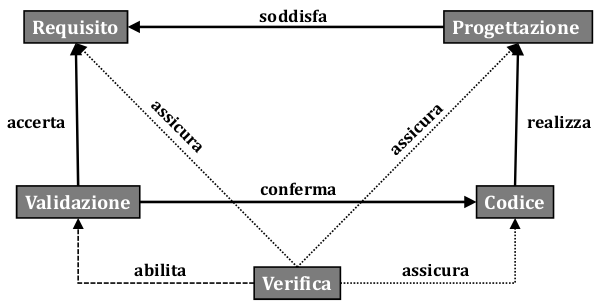
\includegraphics[width=0.7\textwidth]{img/trac}
			\caption{Visualizzazione ordine del tracciamento dei requisiti.}
		\end{figure}

		\textbf{Tracciamento sul codice}: \\ %slide 14/30	  13 dicembre - verifica e validazione: analisi statica
		Il tracciamento è qui vitale perché devo essere sicura di quello che sto facendo e di non fare cose oziose.
		Dimostra completezza ed \underline{\hyperref[economicita]{economicità}} della soluzione e connette sempre parti correlate, infatti ha luoghi su ogni passaggio dello sviluppo (ramo discendente della \underline{\hyperref[V]{figura a V}}) e su ogni passaggio della \underline{\hyperref[verificare]{verifica}} (ramo ascendente).
		Può essere altamente automatizzato.
		Particolari stili di programmazione facilitano il tracciamento, per esempio: assegnare singoli requisiti elementari a singoli moduli del programma richiede una sola \underline{\hyperref[prova]{procedura di prova}} e questo ne semplifica anche la verifica.

	\newpage
	\flushright{\hyperref[index]{\color{black!65}{Ritorna all'indice}}}\flushleft
	\section{U} \label{sec:U}		
	
		\subsection{UNITÀ}	\index{Unità} \label{unita}	
		Divide l'organizzazione del lavoro di programmazione fino al punto in cui non conviene più (corrisponde ad una funzionalità e può essere per esempio una classe o dei dati). Ciò che ho prodotto si chiamano \underline{\hyperref[moduli]{moduli}}. Un unità può essere anche un insieme di più moduli e la specifica di ogni unità architetturale deve essere documentata.
	
		\subsection{USABLE}	\index{Usable}	\label{usable}
		Milestone usable, ovvero il sistema è utilizzare, ha le caratteristiche desiderate, infatti può essere operato dagli utenti. Le funzionalità e le prestazioni richieste sono state verificate e validate e la quantità di difetti è accettabile. Si rivolge alla \underline{\hyperref[productbaseline]{Product Baseline}}.
	
	

	\newpage
	\section{V} \label{sec:V}
	
		\subsection{VALIDARE} \index{Validare} \label{validare}
		\textit{"Did I build the right system?"}. \\ 
		Ha come obiettivo l'accertarsi che il prodotto sia conforme alle attese. (Si fa sull'esito di sviluppo). Prevede \underline{\hyperref[testsistema]{test di sistema}} e \underline{\hyperref[collaudo]{collaudo}}.
		
		\subsection{VALUTAZIONE}
		La qualità fa da appoggio per la valutazione. Varia in base ai destinatari perché hanno diverse aspettative.
		
		\subsection{VERIFICARE} \index{Verificare} \label{verificare}
		\textit{"Did I build the system right?"}. \\
		Accertare che l'esecuzione delle attività di processi svolti nella \underline{\hyperref[fase]{fase}} in esame non abbia introdotto errori nel prodotto. (Fatta rivolta ai processi.) \\
		Esistono diverse forme di verifica:	%set verifica e validazione - introd
		\begin{itemize}
			\item \textbf{Dinamica}: richiede l'esecuzione del programma e si fa tramite \underline{\hyperref[test]{test}};
			\item \textbf{Statica}: non richiede l'esecuzione del prodotto. La più semplice e umana è la lettura. 
			Ci sono due modi di lettura:
			\begin{itemize}
				\item \underline{\hyperref[walkthrough]{Waltkthrough}};
				\item \underline{\hyperref[inspection]{Inspection}}: controllo mirato a cose chiamate lista di controllo;
			\end{itemize}	
		\end{itemize}
		La verifica serve per scovare i problemi e risolverli tempestivamente tramite \textit{\underline{\hyperref[problemsolution]{problem solution}}}. 
		
		\begin{figure}[H]
			\centering
			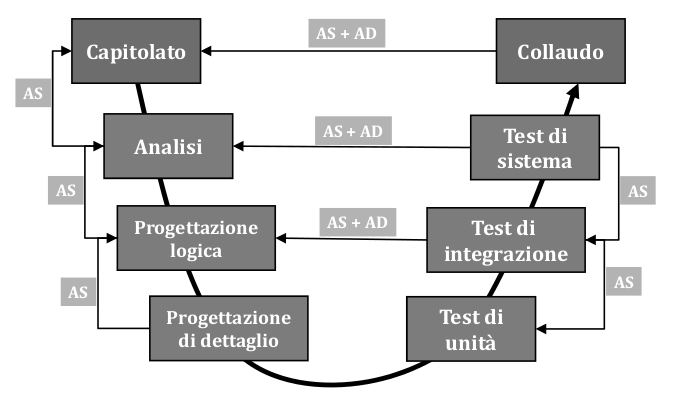
\includegraphics[width=0.6\textwidth]{img/v}		
			\caption{Verifica e validazione nello sviluppo.}
			\label{V}
		\end{figure} 	
		%13 dicembre - verifica e validazione: analisi statica
		La programmazione non deve costituire ostacolo alla verifica, anche se spesso lo fa. L'obiettivo è quindi facilitare la verifica, sebbene esista anche il conflitto tra essere economici (poco) e sapere cosa accade (tanto).
		\textbf{Morale}: serve uno standard di verifica che si protrae in lungo, rendendo agevole la manutenzione, evitando assolutamente la verifica re%V e V: analisi dinamica 20 dicembretrospettiva (ovvero ho fatto e ora rivedo cos'ho fatto). Questo perchè il costo di rilevazione e correzione di errori cresce con l’avanzare dello sviluppo.
		
		\begin{figure}[H]
			\centering
			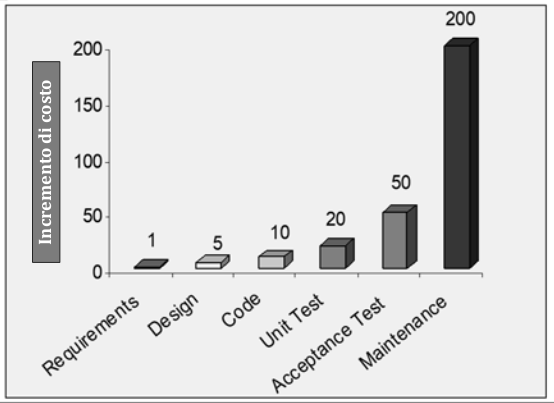
\includegraphics[width=0.6\textwidth]{img/costi}		
			\caption{Costo di correzione di errori.}
		\end{figure} 
		
		Un buon approccio è quindi verificare tramite \underline{\hyperref[byconstruction]{correttezza per costruzione}}. È importante e di nostro interesse scrivere \underline{\hyperref[programmiverificabili]{programmi verificabili}}.
			
		
		\subsection{VERIFICATORE} \index{Verificatore} \label{verificatore}
		È uno dei \underline{\hyperref[ruoli]{ruoli}} in un progetto. Sono presenti per l’intera durata del progetto. Hanno capacità di giudizio e di relazione, oltre ad avere competenze tecniche, esperienza professionale, conoscenza	delle norme.
		
		\subsection{VERSIONE} \index{Versione} \label{versione}
		Software che è in fase di sviluppo. Gli avanzamenti possono a loro volta contenere altri avanzamenti. (Ci sono versioni per ogni parte di una baseline). 
	
	

	\newpage
	\flushright{\hyperref[index]{\color{black!65}{Ritorna all'indice}}}\flushleft
	\section{W} \label{sec:W}
		\subsection{WALKTHROUGH} \index{Walkthrough} \label{walkthrough} %7 dicembre - Verifica e validazione
		Tecnica che consiste nel cercare la presenza di difetti in ogni dove, non sapendo dove. È un metodo di lettura pratico come \underline{\hyperref[inspection]{Inspection}} la cui efficacia dipende dall'esperienza dei verificatori. La strategia, per il codice, prevede il percorrerlo tutto simulandone possibili esecuzioni. \\
		Le sue attività sono divise in 4 e in ognuna svolta deve essere fatta la documentazione:
		\begin{itemize}
			\item fase 1: pianificazione;
			\item fase 2: lettura;
			\item fase 3: discussione;
			\item fase 4: correzione dei difetti;
		\end{itemize}
		
		\subsection{WORK BREAKDOWN STRUCTURE} \index{WBS} \label{wbs}
		È una struttura gerarchica di attività che si compongono di sotto-attività non necessariamente sequenziali e univocamente identificate. 
		%A work-breakdown structure (WBS) in project management and systems engineering, is a deliverable-oriented breakdown of a project into smaller components. A work breakdown structure is a key project deliverable that organizes the team's work into manageable sections.
		
		\begin{figure}[H]
			\centering
			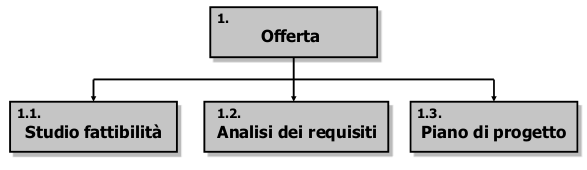
\includegraphics[width=0.8\textwidth]{img/wbs}		
			\caption{Esempio di diagramma di WBS.}
		\end{figure} 
	
	

	% \newpage
	\section{X} \label{sec:X}
	
	

	% \newpage
	\flushright{\hyperref[index]{\color{black!65}{Ritorna all'indice}}}\flushleft
	\section{Y} \label{sec:Y}
	
	

	\newpage
	\section{Z} \label{sec:Z}
	
		\subsection{ZERO-LATENCY} \index{Zero-latency} \label{zero-latency}
		Fare tutto subito (appena l'impegno mi è stato assegnato).
		
		\subsection{ZERO-LAXITY} \index{Zero-laxity} \label{zero-laxity}
		Fare tutto all'ultimo (= zero margine).






%(Allo scritto viene chiesto l'Analisi dei Requisiti. Non ci sarà niente invece riguardo l'implementazione. Ci saranno domande sulle tecniche di verifica)

		%Da inserire:

		%Il caso d'uso ha una funzione esplorativa.


		%26 febbraio 2019 - Misurazione del software - Metodi e obiettivi di quantificazione

		%Idea per metriche: violazioni dello stile di codifica, con grafico a linea diviso per settimane








\end{document}